\documentclass[9pt,twocolumn,twoside]{pnas-new}
\usepackage{gensymb}
\usepackage[colorinlistoftodos]{todonotes}

% new commands:
% q value
\newcommand{\qval}[1]{$q<10^{-#1}$}

% species names
\newcommand{\cel}{\emph{C.~elegans}}
\newcommand{\dicty}{\emph{D.~discoideum}}
\newcommand{\ecol}{\emph{E.~coli}}

% gene names
\newcommand{\gene}[1]{\emph{#1}}

\newcommand{\nlp}{\emph{nlp-31}}
\newcommand{\ftna}{\emph{ftn-1}}
\newcommand{\ftnb}{\emph{ftn-2}}
\newcommand{\cysl}{\emph{cysl-1}}
\newcommand{\nog}{\emph{nog-1}}
\newcommand{\nhr}{\emph{nhr-57}}
\newcommand{\lam}{\emph{lam-3}}

\newcommand{\fog}{\emph{fog-2(lf)}}
\newcommand{\egl}{\emph{egl-9(lf)}}
\newcommand{\rhy}{\emph{rhy-1(lf)}}
\newcommand{\vhl}{\emph{vhl-1(lf)}}
\newcommand{\eglvhl}{\emph{egl-9;vhl-1(lf)}}
\newcommand{\eglhif}{\emph{egl-9;hif-1(lf)}}
\newcommand{\hif}{\emph{hif-1(lf)}}

% protein names
\newcommand{\eglp}{EGL-9}
\newcommand{\rhyp}{RHY-1}
\newcommand{\nogp}{NOG-1}
\newcommand{\vhlp}{VHL-1}
\newcommand{\hifp}{HIF-1}
\newcommand{\fogp}{FOG-2}
\newcommand{\nhrp}{NHR-57}
\newcommand{\lamp}{LAM-3}
\newcommand{\cyslp}{CYSL-1}

% DE genes numbers:
\newcommand{\egln}{1,487}
\newcommand{\rhyn}{1,816}
\newcommand{\vhln}{605}
\newcommand{\eglvhln}{1,989}
\newcommand{\hifn}{481}
\newcommand{\eglhifn}{364}
\newcommand{\fogn}{1,896}
\newcommand{\total}{3,211}
\newcommand{\inall}{53}
\newcommand{\allup}{10}
\newcommand{\alldown}{13}

% downstream targets
\newcommand{\egltargets}{1}
\newcommand{\rhytargets}{0}
\newcommand{\vhltargets}{36}
\newcommand{\hiftargets}{120}
\newcommand{\hifohtargets}{27}

\templatetype{pnasresearcharticle}[9pt,twocolumn,twoside,lineno] % Choose template

\title{Genetic Analysis of a Metazoan Pathway using Transcriptomic Phenotypes}

% Use letters for affiliations, numbers to show equal authorship (if applicable)
% and to indicate the corresponding author
% \author[a,b]{David Angeles-Albores}
% \author[a,b]{Carmie Puckett Robinson}
% \author[a]{Brian Williams}
% \author[b]{Igor Antoshechkin}
% \author[a,b]{Paul W Sternberg}
%
% \affil[a]{Department of Biology and Biological Engineering, Caltech, Pasadena, USA, 91125}
% \affil[b]{Howard Hughes Medical Institute}
% \affil[*]{These authors contributed equally to this manuscript}

% Please give the surname of the lead author for the running footer
\leadauthor{Angeles-Albores}

% Please add here a significance statement to explain the relevance of your work
\significancestatement{
Measurements of global gene expression are often used as
descriptive tools capable of identifying genes that are downstream a
perturbation. In theory, there is no reason why measurements of global
transcriptomes could not be used as a quantitative phenotype for genetic
analysis in multicellular organisms. In fact, qPCR measurements of single or a
few reporter genes are already used to perform genetic network analysis. Here,
we show that transcriptomes can be used for epistasis analysis in a metazoan,
and that transcriptomes afford far more information per experiment than classic
genetic analysis. By using transcriptomes as quantitative phenotypes, we can
accurately predict interactions between genes, while at the same time
identifying genes common to a pathway.
When pathways branch, it is also possible to identify gene batteries that are
associated with each end of the branch point. Finally, genes that would result
in invisible visible phenotypes in an animal are not likely to be invisible at
the transcriptome phenotype due to the exquisite granularity present in these
structures, which represents an important advance towards studying small effect
genes that make up the majority of animals' genetic repertoire.
}

% Please include corresponding author, author contribution and author declaration information
\authorcontributions{
DA, CPR and PWS designed the experiments. CPR selected the
genes and extracted mRNA from all mutants. BW made the libraries. IA performed
all sequencing. DA developed the mathematical theory. DA wrote all computer code
and performed all analyses. DA made all the reporter strains and performed all
microscopy. DA, CPR and PWS wrote the manuscript.
}

\authordeclaration{The authors declare no conflict of interest.}
% \equalauthors{\textsuperscript{1}A.O.(Author One) and A.T. (Author Two)
% contributed equally to this work (remove if not applicable).}
\correspondingauthor{\textsuperscript{2}To whom correspondence should be
addressed. E-mail: pws@caltech.edu}

% Keywords are not mandatory, but authors are strongly encouraged to provide
\keywords{genetics $|$ RNA-Seq $|$ epistasis $|$ hypoxia $|$
          transcriptomics $ | $ systems biology}

\begin{abstract}
RNA-Seq is a technology that is commonly used to identify genetic modules that
are responsive to a perturbation. In theory, global gene expression could also
be used as a phenotype in complex metazoans, with all the implications that has
for genetic analysis. To that end, we sequenced the transcriptome of four single
mutants and two double mutants of the hypoxia pathway in \cel{}. We successfully
analyzed the single mutants in a blinded fashion to predict the genetic
relationships between the genes, and used the double mutants as a test of our
predictions and to infer the directionality of the relationship.
We show that genes along a pathway tend to decorrelate as a result of
alternative regulatory modes and crosstalk with other pathways; and that this
decorrelation accurately reflects functional distance between genes. As a
by-product of our analysis, we predict \hiftargets{} genes under the regulation
of \gene{hif-1}, and \vhltargets{} genes under the regulation of \gene{vhl-1}.
Interactive graphics for this paper
can be found at \url{www.wormlabcaltech.github.io/mprsq}.
\todo[inline]{Abstract must be re-written.}
\end{abstract}

\dates{This manuscript was compiled on \today}
\doi{\url{www.pnas.org/cgi/doi/10.1073/pnas.XXXXXXXXXX}}

\begin{document}

% Optional adjustment to line up main text (after abstract) of first page with
% line numbers, when using both lineno and twocolumn options.
% You should only change this length when you've finalised the article contents.
\verticaladjustment{-2pt}

\maketitle
\thispagestyle{firststyle}
\ifthenelse{\boolean{shortarticle}}{\ifthenelse{\boolean{singlecolumn}}{\abscontentformatted}{\abscontent}}{}

% If your first paragraph (i.e. with the \dropcap) contains a
% list environment (quote, quotation, theorem, definition, enumerate, itemize...),
% the line after the list may have some extra indentation. If this is the case,
% add \parshape=0 to the end of the list environment.
\dropcap{G}enetic analysis of molecular pathways has traditionally been performed
through epistatis analysis. Epistasis occurs when two genes interact, either
directly (biochemical interaction of their gene products) or indirectly. If two
genes interact, and the mutants of these genes have a quantifiable phenotype,
the double mutant of interacting genes will have a phenotype that is not the sum
of the phenotypes of the single mutants that make up its genotype. Epistasis
analysis remains a cornerstone of genetics today~\cite{Phillips2008}.

Recent developments in biology have seen a shift in focus from studying single
genes to -omics methods that measure a property of the biological system
genome-wide. In particular, RNA-seq~\cite{Mortazavi2008} enables biologists to
identify genes that change expression in response to a perturbation. Recent
developments have improved the power and resolution of this technique by enabling
deeper and more frequent sequencing due to lower sequencing costs~\cite{Metzker2010};
better and faster abundance quantification~\cite{Patro2014,Bray2016,Patro2015};
as well as improved differential expression analysis
methods~\cite{Pimentel2016,Trapnell2013}. As a result, RNA-Seq has been
successfully used to identify genetic modules involved in a variety of processes,
including T-cell regulation~\cite{Singer2016,Shalek2013}, the \cel{} linker
cell migration~\cite{Schwarz2012}, or planarian stem cell
maintenance~\cite{VanWolfswinkel2014,Scimone2014}. For the most part, the role of
transcriptional profiling has been restricted to target gene identification.

Although transcriptional profiling has been primarily used for descriptive purposes,
transcriptomic phenotypes have been used to make genetic inferences previously.
Work in \emph{S. cerevisiae} and \dicty{} using microarrays showed
that transcriptomes can be used to infer genetic relationships in simple
eukaryotes~\cite{Hughes2000, VanDriessche2005}. Additionally, eQTL studies in
\cel{} and \emph{Drosophila melanogaster} have established the usefulness of
transcriptomic phenotypes for population genetics studies~\cite{}.
\todo[inline]{Need citations. Maybe add a bit more, it's fluffy.}
In cell culture, single-cell RNA-seq has seen significant progress towards using
transcriptomes as phenotypes with which to test genetic interactions
~\cite{Adamson2016,Dixit2016}.
More recently, we have shown the first identification of a developmental state
of \cel{} using whole-organism transcriptome profiling~\cite{Angeles-Albores2016a}.
To investigate the ability of whole-organism transcriptomes to serve as quantitative
phenotypes for epistasis analysis in metazoans, we sequenced the transcriptomes of
of four well-characterized loss of function mutants in the \cel{} hypoxia
pathway~\cite{Epstein2001,Shen2006,Shao2009,Jiang2001}.

% carmie:
Metazoans depend on the presence of oxygen in sufficient concentrations to
support aerobic metabolism. Genetic pathways evolved to rapidly respond to any
acute or chronic changes in oxygen levels at the cellular or organismal level.
These oxygen sensitive pathways are involved in a broad range of human
pathologies and they have been subject to investigation biochemical and
genetic approaches~\cite{Semenza2012}. These approaches identified the Hypoxia
Inducible Factors (HIFs) as an important group of oxygen responsive genes.

Hypoxia Inducible Factors are highly conserved in metazoans~\cite{Loenarz2011}.
A common mechanism for hypoxia-response induction is heterodimerization between a
HIF$\alpha$ and a HIF$\beta$ subunit. The heterodimer then initiates
transcription of target genes~\cite{Jiang1996}. The number and complexity of HIFs varies
throughout metazoans, with humans having three HIF$\alpha$ subunits and two
HIF$\beta$ subunits, whereas in the roundworm \emph{Caenorhabditis~elegans}
(\cel{}) there is a single HIF$\alpha$ gene, \gene{hif-1}~\cite{Jiang2001} and a single HIF$\beta$
gene, \gene{ahr-1}~\cite{Powell-Coffman1998}. HIF target genes have been implicated
in a wide variety of cellular and extracellular processes such as glycolysis,
extracellular matrix modification, autophagy and immunity~\cite{Semenza1994,
Bishop2004,Shen2005,Bellier2009,Semenza2012}.

Levels of HIF$\alpha$ proteins tend to be tightly regulated. Under conditions of
normoxia, \hifp{}$\alpha$ exists in the cytoplasm and partakes in a futile cycle
of continuous protein production and rapid degradation~\cite{Huang1996}.
\hifp{}$\alpha$ is hydroxylated by three proline hydroxylases
in humans (PHD1, PHD2 and PHD3) but is only hydroxylated by one proline
hydroxylase (\gene{egl-9}) in \cel{}~\cite{Kaelin2008}. \hifp{} hydroxylation
increases its binding affinity to Von Hippel Lindau Tumor Suppressor 1
(\vhlp{}), which allows ubiquitination of \hifp{} leading to its subsequent
degradation. In \cel{}, \eglp{} activity is inhibited by binding of \cyslp{},
and \cyslp{} activity is in turn inhibited at the protein level by \rhyp{},
possibly by post-translational modifications to \cyslp{}~\cite{Ma2012} (see
Fig.~\ref{fig:pathway}).

% heatmap
\begin{figure}[tbhp]
\centering
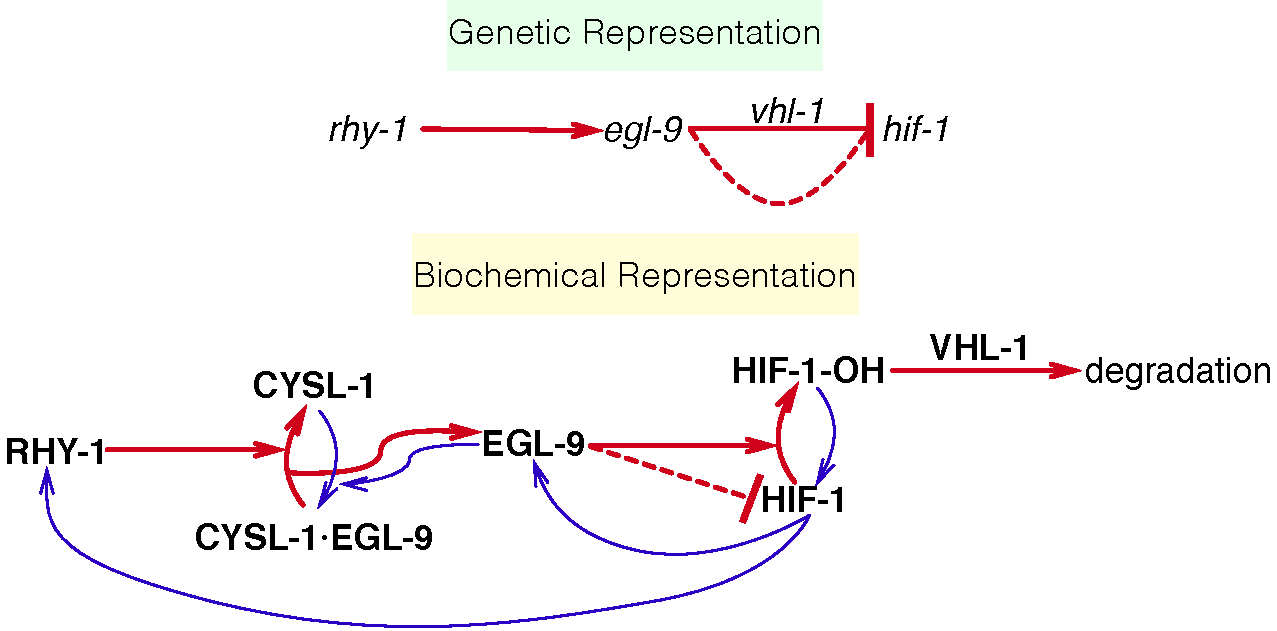
\includegraphics[width=\linewidth]{figs/HIF1pathway.pdf}
\caption{
Genetic and biochemical representation of the hypoxia pathway in \cel{}.
Red arrows are arrows that lead to inhibition of \hifp{}, and blue arrows
are arrows that increase \hifp{} activity or are the result of \hifp{} activity.
\eglp{} is known to exert \gene{vhl-1}-dependent and independent repression
on \hifp{} as shown in the genetic diagram. The biochemical diagram does not
reflect the \gene{vhl-1}-independent repression of \hifp{} by \eglp{} because
that pathway is considerably less well understood.
}
\label{fig:pathway}
\end{figure}

Here, we show that transcriptomes contain strong, robust signals that can be
used to infer relationships between genes in complex metazoans by reconstructing
the hypoxia pathway in \cel{} using RNA-Seq.
Furthermore, we show that the phenomenon of phenotypic epistasis, a hallmark of
genetic interaction, holds at the molecular systems level.
We also demonstrate that transcriptomes contain sufficient information, under
certain circumstances, to order genes in a pathway using only single mutants.
Finally, we were able to identify genes that appear to be downstream of \gene{egl-9}
and \gene{vhl-1}, but do not appear to be targets of \gene{hif-1}.
Using a single set of genome-wide measurements, we were able to observe and
quantitatively assess  significant fraction of the known transcriptional
effects of \gene{hif-1} in \cel{}.
A complete, interactive version of the analysis is also available at
\url{www.wormlabcaltech.github.io/mprsq}.

\section*{Results}
\subsection*{The hypoxia pathway controls thousands of genes in \cel{}}
\label{sub:summary}

We performed whole-organism RNA-seq of the hypoxia pathway at a moderate
sequencing depth ($\sim7$ million mapped reads for each individual replicate)
under normoxic conditions, which allowed us to measure 13,598 isoforms across all
replicates and genotypes, which constitutes over half of all isoforms in \cel{}.
We analyzed our data using a general linear model (see~\ref{methods}) on
logarithm-transformed counts. Changes in gene expression are quantified via a
regression coefficient, $\beta$ which is specific to each isoform within a genotype.
Statistical significance is achieved when the q-values for each $\beta$ (p-values
adjusted for multiple testing) are less than 0.1. Genes that are significantly
altered between wild-type and a given mutant have $\beta$ values that are
statistically significantly different from 0.  These coefficients are not equal
to the average log-fold change per gene, although they are loosely related to
this quantity. Larger magnitudes of $\beta$ correspond to larger perturbations.
These coefficients can be used to study the RNA-Seq data in question.

In spite of the moderate sequencing depth, transcriptome profiling of the hypoxia
pathway revealed that this pathway controls thousands of genes in \cel{}. The
\egl{} transcriptome showed differential expression of \egln{} genes, similarly to
the \rhyn{} genes differentially expressed in \rhy{} mutants. The \vhl{}
transcriptome showed considerably fewer differentially expressed genes (\vhln{}),
possibly reflecting the known fact that it is a weaker controller of \hif{} than
\egl{}~\cite{Shao2009}. The \egl{};\vhl{} double mutant transcriptome showed
\eglvhln{} differentially expressed genes. The \hif{} mutant also showed a
transcriptomic phenotype involving \hifn{} genes. The \eglhif{} double mutant
showed a similar number of genes with altered expression (\eglhifn{}).

% \subsection*{Clustering visualizes epistatic relationships between genes}
% \label{sub:Clustering}
%
% As a first step in our analysis, we analyzed our data using a general
% linear model (see~\ref{methods}) on logarithm-transformed
% counts. Genes that are significantly altered between wild-type and a given
% mutant have a genotype coefficient ($\beta$) that is statistically significantly
% different from 0. We refer to these coefficients through the greek letter. These
% coefficients are not identical to the average log-fold change per gene, although
% they are loosely related to this quantity. Larger magnitudes of $\beta$
% correspond to larger perturbations. These coefficients can be used to study the
% RNA-Seq data in question.
%
% Clustering is a well-known technique in bioinformatics that is used to identify
% relationships between high dimensional data points~\cite{Yeung2003}. We wanted
% to make sure that clustering by differential expression yielded genetically
% relevant information. \hif{} exhibits no obvious phenotypes under normoxic
% conditions, in contrast to \egl{}, which exhibits an egg-laying (Egl)
% phenotype in the same environment. \eglhif{} mutants suppress the
% Egl phenotype. If transcriptomic phenotypes correlate with their identified
% phenotypes, \hif{} should cluster with the \eglhif{} double
% mutant, whereas \egl{} should cluster away from the \hif{} mutant.
% Indeed, when blind, unsupervised clustering was performed on the data, three
% clusters emerged. \hif{} and \eglhif{} clustered together, indicating
% suppression of the \egl{} phenotype; whereas \egl{}, \eglvhl{}, \vhl{} and
% \rhy{} all clustered separately. Finally, our negative control \fog{} was in its
% own cluster (see Fig.~\ref{fig:dendrogram}). We conclude that expression profiling
% measures enough signal to cluster genes in a meaningful manner in complex
% metazoans.
%
% % dendrogram
% \begin{figure}%[tbhp]
% \centering
% 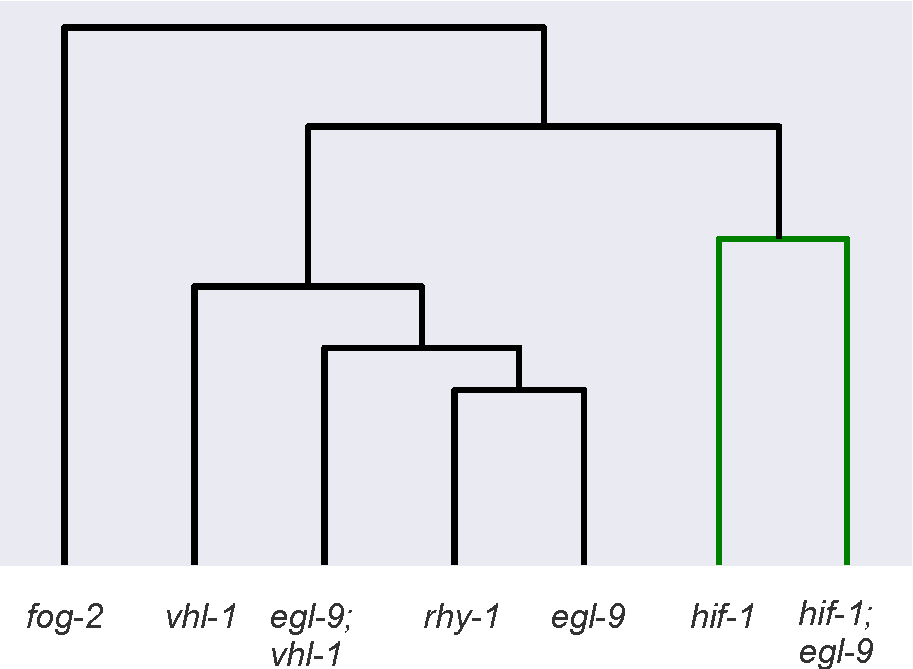
\includegraphics[width=0.75\linewidth]{figs/dendrogram.pdf}
% \caption{
% Unsupervised aggregative clustering of various \cel{} mutants. Genes
% cluster in a manner that is biologically intuitive. Genotypes that have an
% activated hypoxia response (i.e, \egl{}, \vhl{}, and \rhy{}) cluster far
% from \hif{}. \hif{} clusters with the suppressed \eglhif{} double mutant.
% The \fog{} transcriptome, used as an outgroup, clusters farthest away.
% }
% \label{fig:dendrogram}
% \end{figure}

\subsection*{Principal Component Analysis visualizes epistatic relationships between genotypes}
\label{sub:Clustering}

Principal Component Analysis (PCA) is a well-known technique in bioinformatics that is
used to identify relationships between high dimensional data points\todo[inline]{
Need new citation for PCA
}
% ~\cite{Yeung2003}
We performed PCA on our data to examine whether each genotype clustered in a biologically
relevant manner. We expected \hif{} to cluster near \eglhif{}, because
\hif{} exhibits no obvious phenotypes under normoxic conditions, in contrast to
\egl{}, which exhibits an egg-laying (Egl) phenotype in the same environment.
\eglhif{} mutants suppress the Egl phenotype and exhibit the \hif{} (wild-type) phenotype
instead. On the other hand, we expected \egl{}, \rhy{}, \vhl{} and \eglvhl{} to
form a separate cluster since each of these genotypes is Egl and has a constitutive
hypoxic response. Finally, we expected that \fog{}, which we included as a negative
control, should appear far away from either cluster.

The first dimension of the PCA analysis was able to discriminate between \hifp{}
positive and negative animals, whereas the second dimension was able to discriminate
between mutants within the hypoxia pathway and outside the hypoxia pathway.
Therefore expression profiling measures enough signal to cluster genes in a
meaningful manner in complex metazoans.

% dendrogram
\begin{figure}%[tbhp]
\centering
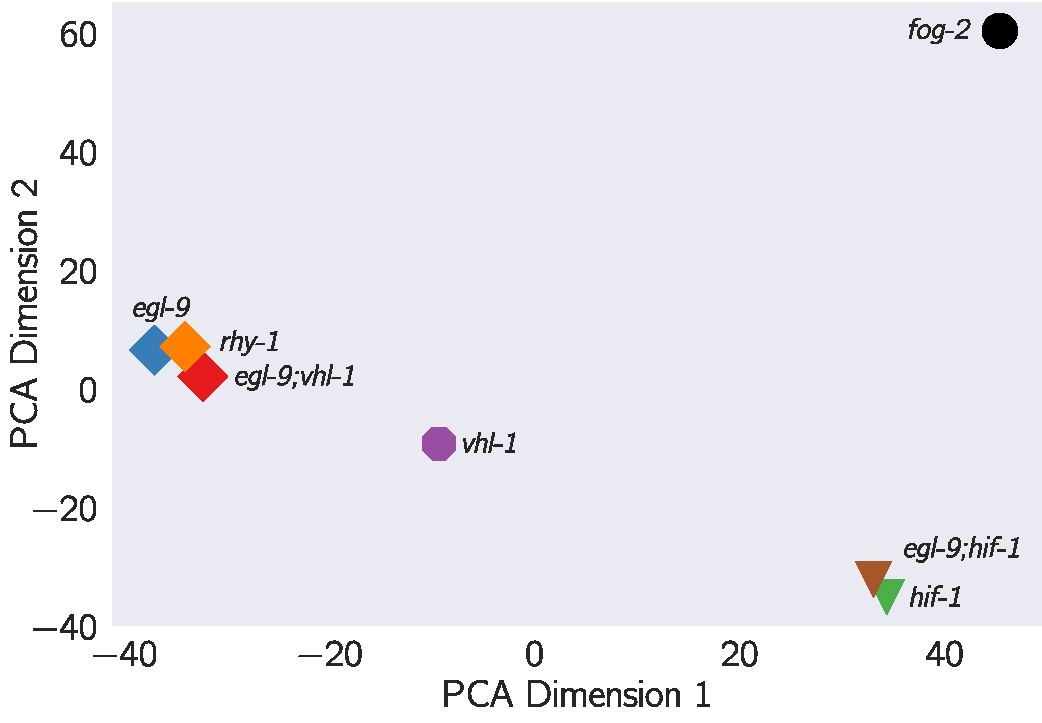
\includegraphics[width=0.75\linewidth]{figs/pca.pdf}
\caption{
Principal component analysis of various \cel{} mutants. Genotypes that have an
activated hypoxia response (i.e, \egl{}, \vhl{}, and \rhy{}) cluster far
from \hif{}. \hif{} clusters with the suppressed \eglhif{} double mutant.
The \fog{} transcriptome, used as an outgroup, is far away from either cluster.
}
\label{fig:dendrogram}
\end{figure}


\subsection*{Reconstruction of the hypoxia pathway from first genetic principles}
\label{sec:reconstruct}
Having shown that the signal in the mutants we selected was strong enough to
cluster mutants using the regression coefficients, we set out to reconstruct the
hypoxia pathway from first genetic principles. In general, to reconstruct a pathway,
we must assess whether two genes act on the same phenotype (independence);
then we must measure whether these genes act additively or epistatically on the
measured phenotype; and if there is epistasis we must measure whether it is positive
or negative, in order to assess whether the epistatic relationship is a genetic
suppression or a synthetic interaction.

\subsubsection{Genes in the hypoxia mutant act on the same transcriptional phenotype}
\label{sec:phenotypes}
We observed that all the hypoxia mutants had significant overlap between their
differentially expressed transcriptomes relative to a wild-type control
(fraction of shared transcriptomes ranged from a minimum of 65 genes
shared between \hif{} and \eglhif{} to a maximum of 1,249 shared genes between
\egl{} and \eglvhl{}). For comparison, we also analyzed a previously published
\fog{} transcriptome~\cite{Angeles-Albores2016a}. The \gene{fog-2} gene is
involved in masculinization of the \cel{} germline, which enables sperm formation,
and is not known to be involved in the hypoxia pathway. The hypoxia
pathway transcriptomes and the \fog{} transcriptome showed significant overlap
(123--618 genes). Given the similar overlaps between known interactors and an
unknown transcriptome, we conclude that the \fog{} mutant we studied acts on the
same phenotype as mutants from the hypoxia pathway.

% genetic correlations
\begin{figure}%[tbhp]
\centering
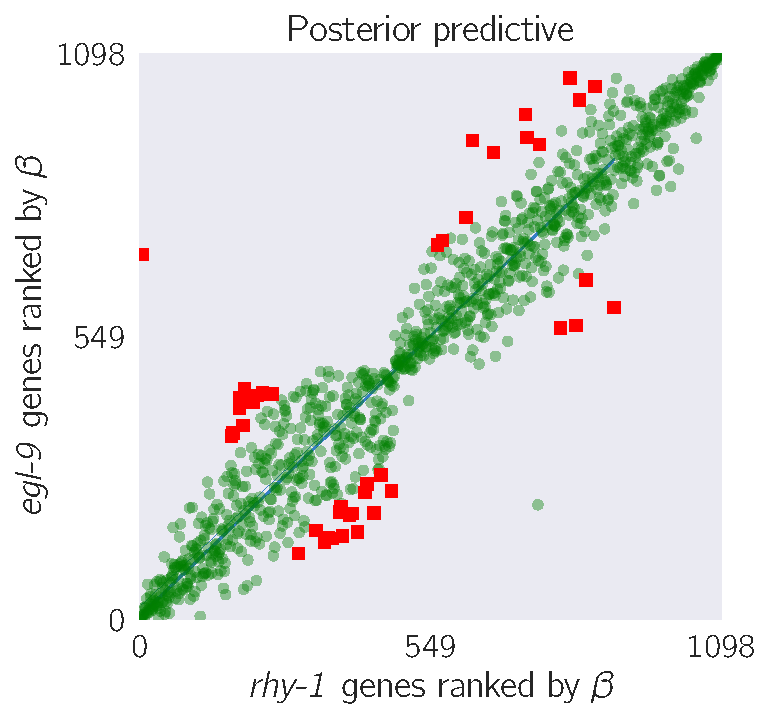
\includegraphics[width=\linewidth]{figs/multiplemodes-eb.pdf}
\caption{
Strong transcriptional correlations can be identified between genes
that share a positive regulatory connection. We took the \egl{} and the \rhy{}
transcriptomes, identified differentially expressed genes common to both
transcriptomes and ranked each gene according to its differential expression
coefficient $\beta$. We plotted the rank of each gene in \rhy{} versus the
rank of the same gene in the \egl{} transcriptome. The result is an almost
perfect correlation. Green, transparent large points mark inliers to the primary
regressions (blue lines); red squares mark outliers to the primary regressions.
}
\label{fig:genetic_interactions}
\end{figure}

Although overlapping transcriptomes may be enough to conclude that a set of mutants
share a phenotype, we wanted to know whether it was informative to
look at quantitative agreement between perturbations. We rank-transformed
the regression coefficients $\beta$ for each transcriptome, and calculated lines
of best fit using Bayesian regression with a Student-T distribution to mitigate
noise from outliers (see Fig~\ref{fig:genetic_interactions}). For transcriptomes
associated with the hypoxia pathway, we found that these correlations tended to have
values higher than 0.9 with a tight distribution around the line of best fit.
The correlations for mutants from the hypoxia pathway
with the \fog{} mutant were considerably weaker, with magnitudes between
0.6--0.85 and a greater variance around the line of best fit.
Although \gene{hif-1} is known to be genetically repressed by \gene{egl-9}, \gene{rhy-1} and
\gene{vhl-1}~\cite{Epstein2001,Shen2006}, all the correlations
between mutants of these genes and \hif{} were positive. The overlap between
\hif{} and all other mutants was small, and each overlap involved
different sets of genes, which suggests that we did not sequence deeply enough
to identify the nature of these positive interactions.
After we calculated the pairwise correlation between each transcriptome,
we weighted the result of each regression by the
number of differentially expressed isoforms shared by two transcriptomes and
divided by the total number of differentially expressed isoforms present in the
two transcriptomes, $N_\mathrm{overlap}/N_{\mathrm{g_1} \cup \mathrm{g2}}$.
The weighted regressions recapitulated a network with three `modules': A control
module, a responder module and an uncorrelated module (see Fig.~\ref{fig:heatmap}).
We identified a strong positive interaction between \egl{} and \rhy{}.
The magnitude of this weighted correlation derives from the magnitude of the
transcriptomes for these mutants (\egln{} and \rhyn{} differentially expressed
genes respectively) and the overlap between both genes was
extensive, which makes the weighting factor considerably larger than other pairs.
The weak correlation between \hif{} and \egl{} is derived from the small size of
the \hif{} transcriptome and the small overlap between the transcriptomes.
% Likewise, the weak correlation between \hif{} and \egl{}, \vhl{} and \rhy{} is at
% least partially the result of its relatively weak transcriptomic phenotype relative
% to the other genes, particularly \egl{} and \rhy{}.
The fine-grained nature of transcriptional phenotypes means that these weighted
correlations between transcriptomes of single mutants are predictive of genetic
interaction.

% heatmap
\begin{figure}[tbhp]
\centering
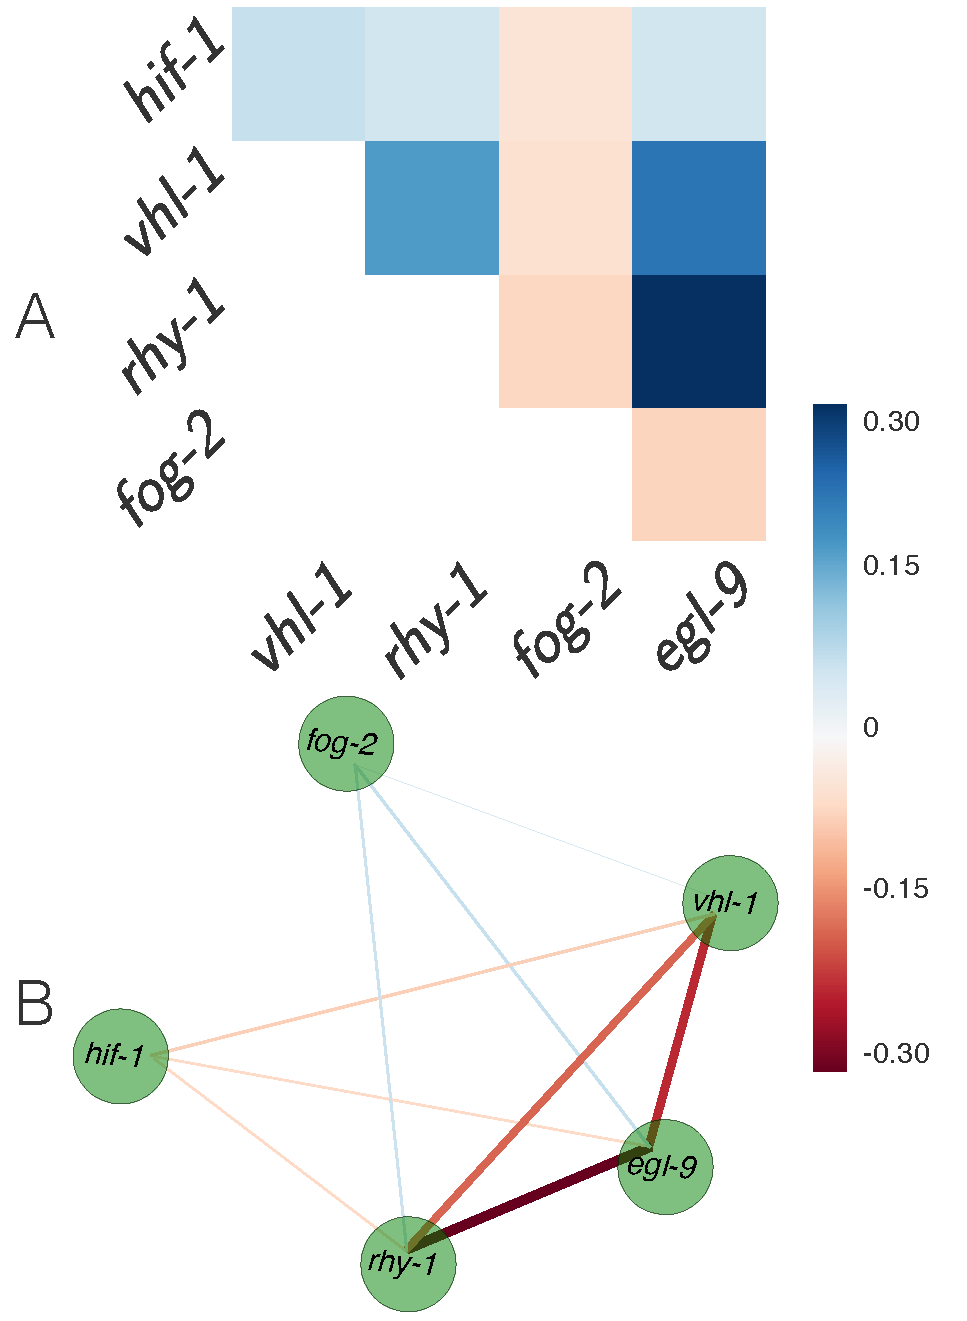
\includegraphics[width=\linewidth]{figs/bayesian_heat_map.pdf}
\caption{
\textbf{A}: Heatmap showing pairwise regression values between all
single mutants. \textbf{B}: Correlation network drawn from the diagram. Edge
width is proportional to the logarithm of the magnitude of the weighted
correlation between two nodes divided by absolute value of the weighted
correlation value of smallest magnitude. Edges are also colored according to the
heatmap in \textbf{A}.
}
\label{fig:heatmap}
\end{figure}

\subsubsection*{A quality check of the transcriptomic data reveals excellent agreement
            with the literature}
\label{sub:quality_check}
One way to establish whether genes are acting additively or epistatically to each
other is to perform qPCR of a reporter gene in the single and double mutants. This
approach was used to successfully map the relationships within the hypoxia
pathway (see, for example~\cite{Shao2009,Shen2006}). A commonly used reporter is
\nhr{}, which is known to exhibit a several fold increase in mRNA expression when
\hifp{} accumulates\cite{Shen2006,Shen2005,Ackerman2012,
Park2012}. Likewise, \hifp{} is known to increase transcription of \gene{rhy-1}
and \gene{egl-9}~\cite{Powell-Coffman2010}.

Our dataset enables us to perform an equivalent computational experiment to qPCR
by selectively looking at expression of a few genes at a time. Therefore, we
queried the changes in expression of \gene{rhy-1}, \gene{egl-9}, \nhr{}. We included
\lam{} as a representative negative control. In our dataset, \nhr{} is upregulated in
\egl{}, \rhy{} and \vhl{}, but remains unchanged in \hif{}.
\eglvhl{} had an expression level similar to \egl{}; whereas the
\eglhif{} mutant showed wild-type levels of the reporter expression, as reported
previously~\cite{Shen2006}.

% in silico qPCR
\begin{figure}[tbhp]
\centering
\includegraphics[width=\linewidth]{figs/qpcr.pdf}
\caption{
\textbf{Top}: \emph{In silico} qPCR.\@ We extracted
four genes (\gene{rhy-1}, \gene{egl-9}, \nhr{} and \lam{}, shown on the x-axis)
and plotted their regression coefficients, $\beta$, as measured for every
genotype (represented by one of six colors) to study the epistatic relationships
between each gene. Stars above a bar represent a regression coefficient
statistically significantly different from 0, meaning that expression is altered
relative to a wild-type control. Error bars show standard error of the mean
value of $\beta$. \nhr{} is an expression reporter that has been used previously
to identify \gene{hif-1} regulators~\cite{Shen2006,Shao2009}. The \nhr{} mRNA
levels replicate what is observed in the literature. \lam{} is shown here as a
negative control that should not be altered by mutations in this pathway. The
increases in the levels of \gene{egl-9} and \gene{rhy-1} when repressors of
\gene{hif-1} are knocked out are in agreement with previous
literature~\cite{Powell-Coffman2010}. We measured modest increases in the levels
of \gene{rhy-1} mRNA when \hif{} is knocked out. The mechanism behind this is
unclear. Negative and positive feedback loops from \gene{hif-1} into its
inhibiting genes could be a homeostatic mechanism.
}
\label{fig:qpcr}
\end{figure}

We also performed \emph{in silico} qPCR of every gene under scrutiny to get a
clearer idea of the relationships between them (see Fig.~\ref{fig:qpcr}). We
observed changes in \rhy{} expression consistent with previous
literature~\cite{Shen2006} when \hifp{} accumulates.
We also observed changes in \gene{egl-9} expression in \egl{}.
\gene{egl-9} is known as a hypoxia responsive gene~\cite{Powell-Coffman2010}.
Although changes in \gene{egl-9} expression were not statistically significantly
different from the wild-type in
\rhy{} and \vhl{} mutants, the mRNA levels of \gene{egl-9} still trended towards
increased expression in these genotypes. As with \nhr{}, \gene{egl-9} and
\gene{rhy-1} expression was wild-type in \eglhif{}; whereas \eglvhl{}
mutant showed expression phenotypes identical to \egl{}. This dataset also showed
that knockout of \gene{hif-1} resulted in a modest increase in
the levels of \gene{rhy-1}. This suggests that \gene{hif-1}, in addition to being
a positive regulator of \gene{rhy-1}, also inhibits it, which constitutes a novel
observation. Taken together, these results indicate that RNA-seq data is
equivalent to qPCR for purposes of comparing gene expression of a reporter between
genotypes. Using a single reporter we would have been able to reconstruct an
important fraction of the genetic relationships between the genes in the hypoxia
pathway.

% \subsection*{Genes in the hypoxia pathway exhibit genome-wide epistasis}
\subsection*{Genome-wide epistasis}
Although it may be sufficient to extract the regression coefficients of a
known reporter gene and use it to rebuild a genetic pathway, we felt that by
relying on just a single gene, or even a handful of genes to rebuild the pathway
we discarded most of the valuable information present in RNA-seq datasets. Therefore,
we decided to explore a new epistasis metric---genome-wide epistasis.

Ideally, any measurement of genome-wide epistasis should conform to certain
expectations. First, it should make use of the regression coefficients of as
many genes as possible. Second, it should be summarizable in a single,
well-defined number. Third, it should have an intuitive behavior, such that
the special values of the statistic (maximum, minimum, zero) should have an
unambiguous interpretation.

One way of defining genome-wide epistasis is to plot transcriptome data onto
an epistasis plot. In an epistasis plot, the X-axis represents the
expected expression of a double mutant $X^-Y^-$ if $X$ and $Y$ interact additively.
In other words, it is the sum of the regression coefficients for an isoform
calculated from the single mutants $X^-$ and $Y^-$. The Y-axis represents the
deviations from the additive (null) model, and
can be calculated as the difference between the observed regression coefficient
and the predicted regression coefficient. Only genes that are differentially
expressed in all three genotypes are plotted.

Epistasis plots can be understood intuitively for simple cases of genetic
interactions. If two genes act additively on the same set of differentially expressed
isoforms then all the plotted points will fall along the line $y=0$.
If two genes interact in a single, unbranched pathway, then $X^-$ and $Y^-$ should
have identical phenotypes for $X^-$, $Y^-$ and $X^-Y^-$, if all the genotypes are
homozygous for complete loss of function mutations~\cite{Huang2006}. It follows that the
data points should fall along a line with slope equal to $-\frac{1}{2}$. On the
other hand, in the limit of complete inhibition of $Y$ by $X$, the plots should show
a line of best fit with slope equal to $-1$\footnote{Specifically, this follows
from assuming that $Y^-$ is wild-type under the conditions assayed; and
$X^-Y^-$ = $Y^-$ = wild-type}.
Genes that have a synthetic interaction between them will fall along lines
with slopes $>0$. When there is epistasis of one gene over another, the points will
fall along a line of best fit with slope $s_{XY=Y}$ or $s_{XY=X}$. This slope must
be determined from the single-mutant data.
From this information, we can use the single mutant data to
predict the distribution of slopes that results for each case stated above, as well
as for each epistatic combination ($X^-Y^-=X^-$ or $X^-Y^-=Y^-$). Given the biological
relevance of the slope of the lines of best fit to the biological relationship
between the genes under study, we refer to it as the genome-wide epistasis
coefficient ($s_{X, Y}$), because it integrates information from many different
genes into a single number (see Fig.~\ref{fig:egl9epistasis}).

In our experiment, we studied two double mutants, \eglhif{} and \eglvhl{}.
We wanted to understand how well the global epistasis agreed with the literature
based on qPCR of single reporters. Therefore, we performed orthogonal distance
regression on to the two gene combinations we studied (\gene{egl-9} and \gene{vhl-1};
and \gene{egl-9} and \gene{hif-1}) to determine the epistasis coefficient for each
gene pair. We also generated models for the epistasis cases mentioned above using
the single mutant data. For every simulation, as well as for the observed data,
we used bootstraps to generate probability distributions of the epistasis
coefficients.

When we compared the predictions for the genome-wide epistasis coefficient,
$s_{egl-9,vhl-1}$ under different assumptions with the observed slope ($-0.42$). We
observed that the predicted slope matched the simulated slope for the case where
\gene{egl-9} is epistatic over \gene{vhl-1} (\egl{} = \eglvhl{}, see
Fig.~\ref{fig:egl9epistasis}) and did not overlap with any other prediction.
Next, we predicted the distribution of $s_{egl-9,hif-1}$ for different pathways
and contrasted with the observed slope. In this case, we saw that the uncertainty
in the observed coefficient overlapped significantly with the strong suppression
model, where \eglp{} strongly suppresses \hifp{}, and also with the model where
\hif{} = \eglhif{}. In this case, both models are reasonable---\hifp{} is strongly
suppressed by \eglp{}, and we know from previous literature that the epistatic
relationship, \hif{} = \eglhif{}, is true for these mutants. In fact, as the
repression of \hifp{} by \eglp{} becomes stronger, the epistatic model should converge
on the limit of strong repression.

Another way to test which model best explains the epistatic relationship between
\gene{egl-9} and \gene{vhl-1} is to use Bayesian model selection to calculate
an odds ratio between two models to explain the observed data. Models can be placed
into two categories: parameter-free and fit. Parameter free models are `simpler'
because their parameter space is smaller (0 parameters) than the fit models ($n$
parameters). By Occam's razor, simpler models should be preferred to more
complicated models. However, simple models suffer from the drawback that
systematic deviations from them cannot be explained or accomodated, whereas more
complicated models can alter the fit values to maximize their explanatory power.
In this sense, more complicated models should be preferred when the data shows
systematic deviations from the simple model. Odds-ratio selection gives us a way
to quantify the trade-off between simplicity and explanatory power.

We reasoned that comparing a fit model ($y = \alpha\cdot x$, where $\alpha$ is
the slope of best fit) against a parameter-free model ($y = \gamma\cdot x$,
where $\gamma$ is a single number) constituted a conservative approach towards
selecting which theoretical model (if any) best explained the data. In particular,
this approach will tend to strongly favor the line of best fit over simpler model
for all but very small, non-systematic deviations. We decided
that we would reject the theoretical models only if the line of best-fit
was $10^3$ times more likely than the theoretical models (odds ratio, OR $>10^3$).
Comparing the odds-ratio between the line of best fit and the different pathway
models for \gene{egl-9} and \gene{vhl-1} showed similar results to the simulation.
Only the theoretical model \egl{} = \eglvhl{} could not be rejected (OR = 0.02),
whereas all other models were significantly less likely than the line of best fit
(OR $>10^{42}$).
Therefore, \gene{egl-9} is epistatic to \gene{vhl-1}. Moreover,
since $s_{egl-9, vhl-1}$ is strictly between and not equal to $0$ and $-0.5$, we
conclude that \gene{egl-9} acts on its transcriptomic phenotype in
\gene{vhl-1}-dependent and independent manners. A branched pathway that can lead
to epistasis coefficients in this range is a pathway where \gene{egl-9} interacts
with its transcriptomic phenotype via branches that have the same valence (both
positive or both negative)~\cite{Shao2009}. When we performed a similar analysis
to establish the epistatic relationship between \gene{egl-9} and \gene{hif-1},
we observed similar results. All models were rejected (OR $>10^{25}$) except for
the model where \gene{hif-1} is epistatic over \gene{egl-9}.

% epistasis graph
\begin{figure}[tbhp]
\centering
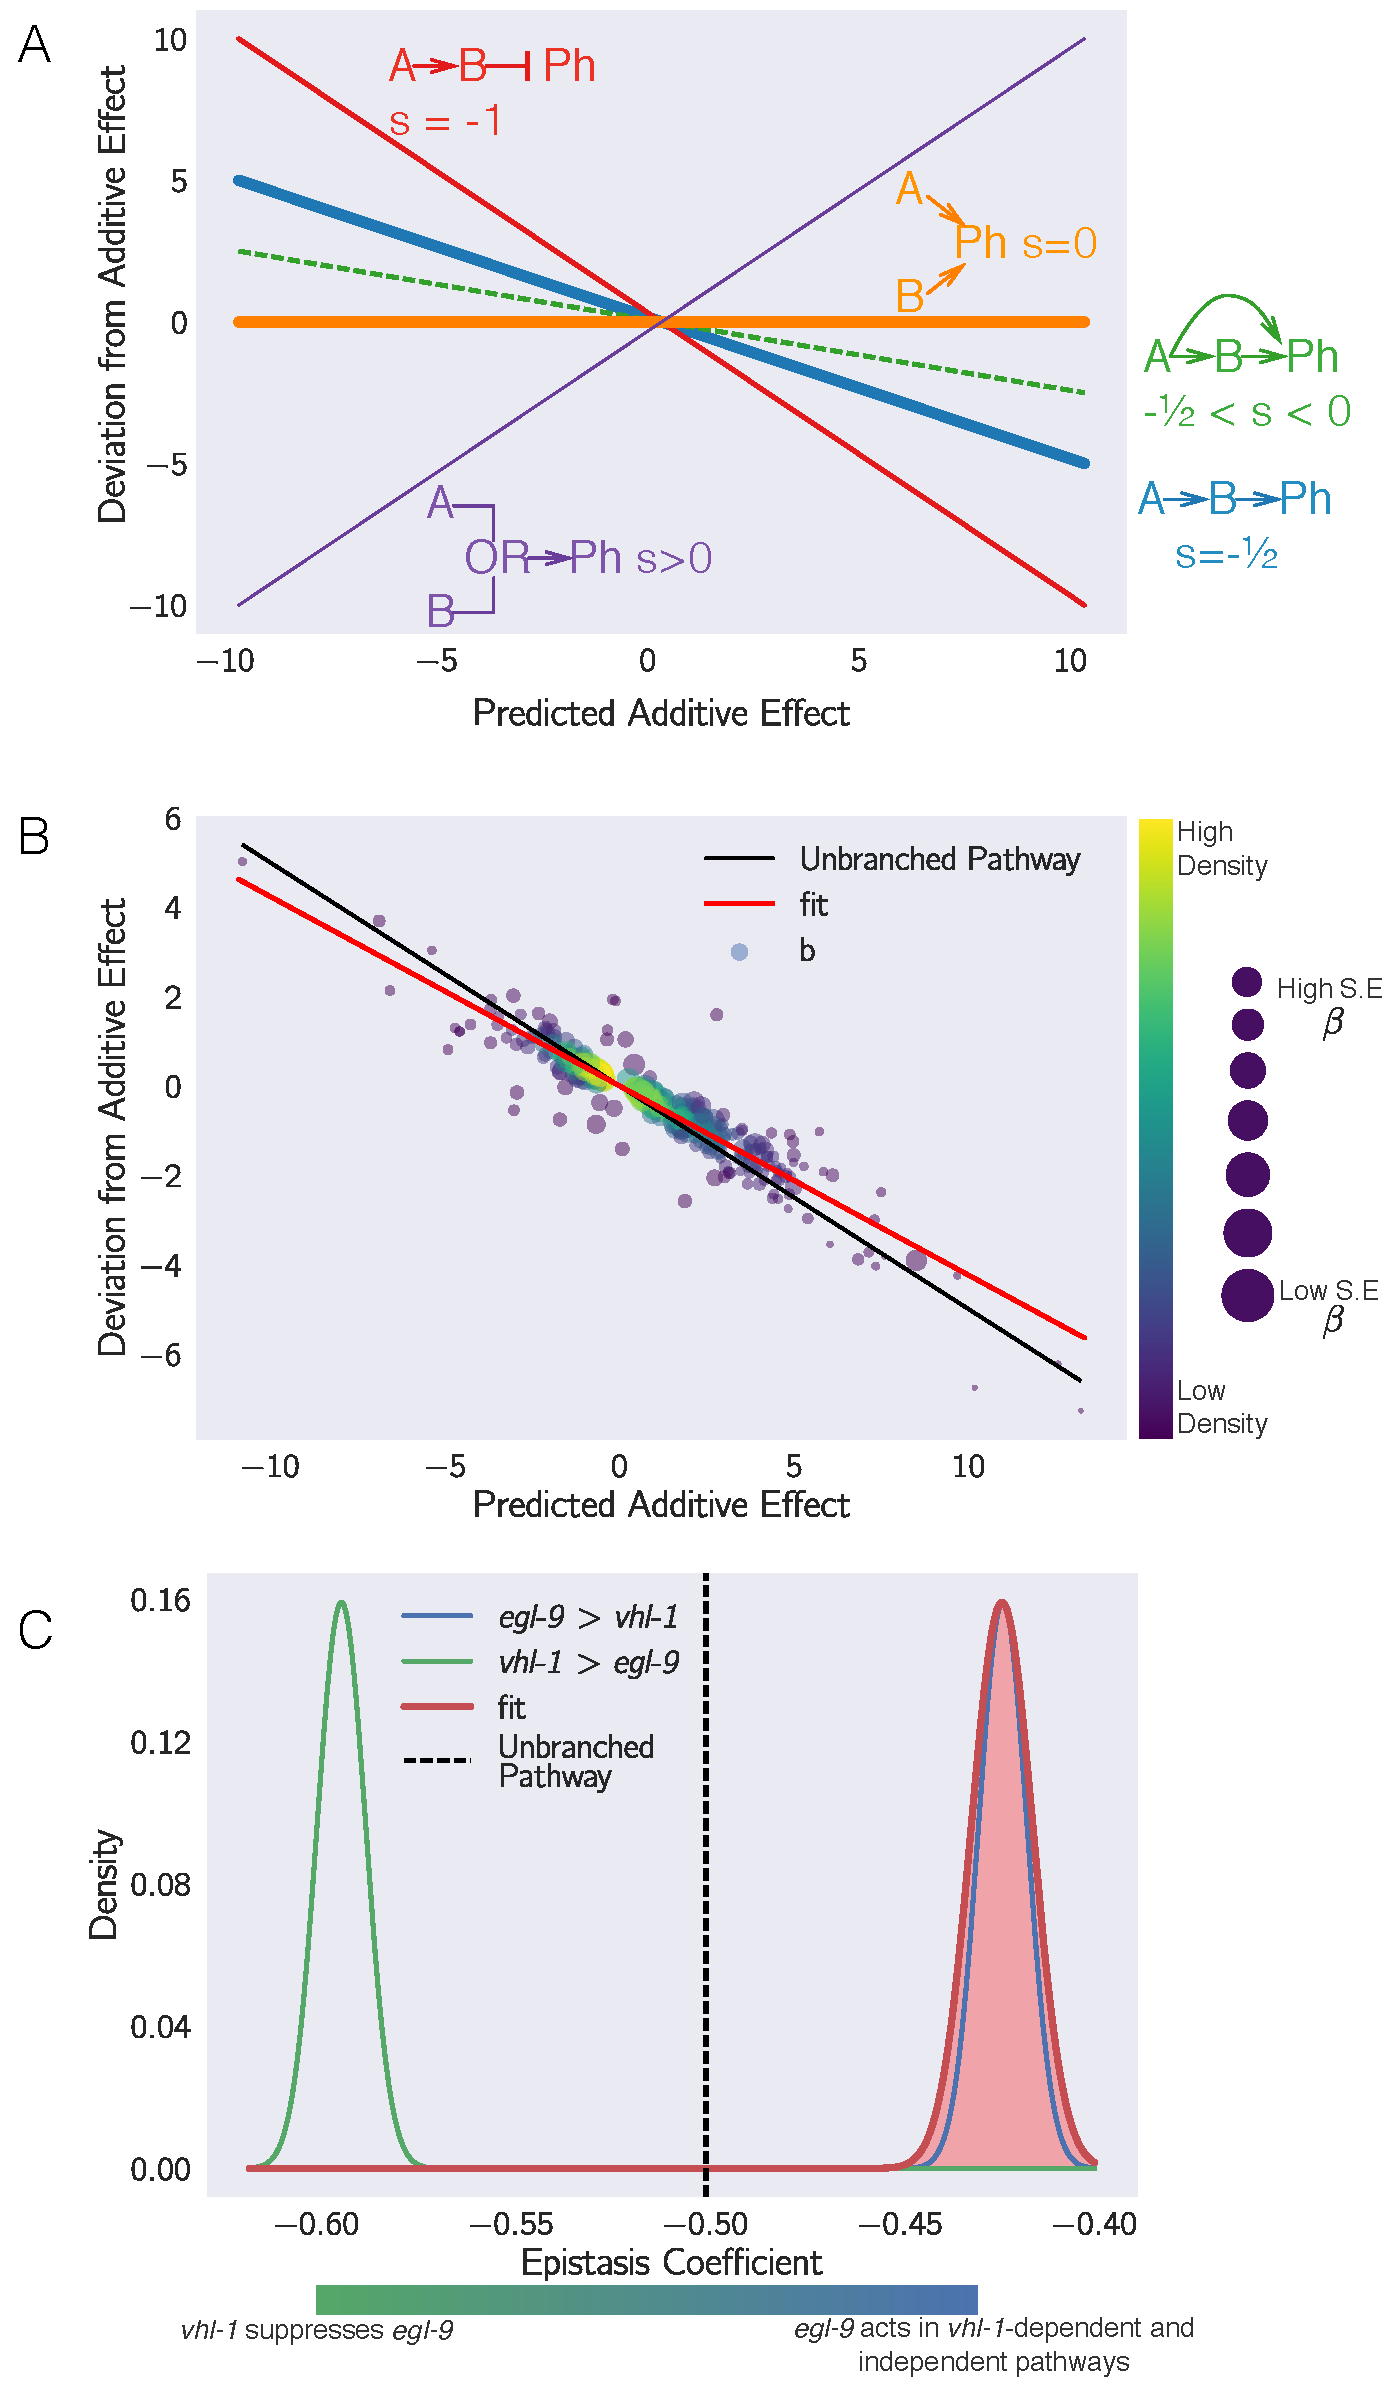
\includegraphics[width=\linewidth]{figs/egl9hif1-epistasis.pdf}
\caption{
(\textbf{A}) Schematic diagram of an epistasis plot. The X-axis on an epistasis
plot is the expected coefficient for a double mutant under an additive model (null model).
The Y-axis plots deviations from this model. Double mutants that deviate in a
systematic manner from the null model exhibit genome-wide epistasis ($s$). To
measure $s$, we perform a linear regression on the data. The slope of the line
of best fit is $s$. This coefficient is related to genetic architectures. Genes
that act additively on a phenotype \textbf{(Ph)} will have $s=0$; whereas genes that act
along a single unbranched pathway will have $s=-1/2$. Strong repression
is reflected by $s=-1$. Cases where $s>0$ correspond to synthetic interactions,
and in the limit as $s\rightarrow\infty$, the synthetic interaction is most likely
to represent an OR-gate. Cases where $0 < s < -1/2$ correspond to circuits
that have positive branches; whereas cases where $-1/2 < s < -1$
correspond to cases where the branches have different valency. Cases where
$s < -1$ represent inhibitory branches.
(\textbf{B}) Epistasis plot showing
that the \eglvhl{} transcriptome deviates significantly from a null additive.
Points are colored qualitatively according to density (purple---low,
yellow---high) and size is inversely proportional to the standard
error of the y-axis (larger points, higher accuracy). The purple line
is the line of best fit from an orthogonal distance regression.
(\textbf{C}) Bootstrapped cumulative
density function for the observed genome-wide epistasis coefficient for
\gene{egl-9} and \gene{vhl-1}. Dashed purple line shows the mean value of the
data. Using the single mutants, we simulated coefficient
distributions for a linear model; an additive model; a model where either
\gene{egl-9} or \gene{vhl-1} suppresses the other gene strongly and epistasis
models where the double mutant has a phenotype equal to one of the single mutants.
We find that the double mutant matches the predicted epistasis curve for
\eglvhl{} = \egl{} (orange and purple). The lack of overlap
between the purple/blue curve (observed epistasis) and the distribution for the
linear pathway strongly suggests that \eglp{} acts on \hifp{} in
\gene{vhl-1}-dependent and independent ways.
}
\label{fig:egl9epistasis}
\end{figure}

\subsubsection*{Epistasis can be predicted}
Given our success in measuring epistasis coefficients, we wanted to know whether
we could predict the epistasis coefficient between \gene{egl-9} and \gene{vhl-1}
in the absence of the \egl{} genotype. Since \rhyp{} activates
\eglp{}, the \rhy{} transcriptome should contain more or less
equivalent information to the \egl{} transcriptome. Therefore, we generated
predictions of the epistasis coefficient between \gene{egl-9} and \gene{vhl-1}
by substituting in the \rhy{} data. We predicted $s_{rhy-1,vhl-1} = -0.45$.
Similarly, we used the \eglvhl{} double mutant to
measure the epistasis coefficient while replacing the \egl{} dataset with the \rhy{}
dataset. We found that the epistasis coefficient using this substitution was $-0.40$.
This coefficient was different from $-0.50$ (OR $>10^{62}$), reflecting the same
qualitative conclusion that the hypoxia pathway is branched.
In conclusion, we were able to obtain a quantitatively close prediction of the
epistasis coefficient for two mutants using the transcriptome of a related,
upstream mutant. Finally, we showed that in the absence of a single mutant, an
upstream locus can under some circumstances be used to estimate epistasis
between two genes.

\subsection*{Transcriptomic decorrelation can be used to infer functional distance}
\label{sub:decorrelation}

We were interested in figuring out whether RNA-Seq could be used to identify
functional interactions within a genetic pathway. Although there is no \emph{a
priori} reason why global gene expression should reflect functional interactions,
the strength of the unweighted correlations between genes in the hypoxia pathway
made us wonder how much information can be extracted from this dataset. Single
genes are often regulated by multiple independent sources. The connection between
two nodes can in theory be characterized by the strength of the edges connecting
them (the thickness of the edge); the fraction of sources that regulate both
nodes (the fraction of common inputs); and the fraction of genes that are
regulated by both nodes (the fraction of common outputs).
In other words we expected that expression profiles associated with a pathway
would respond quantitatively to quantitative changes in activity of the pathway.
Targeting a pathway at multiple points would lead to expression profile
divergence as we compare nodes that are separated by more degrees of freedom,
reflecting the flux in information between them.

% decorrelation
\begin{figure}[tbhp]
\centering
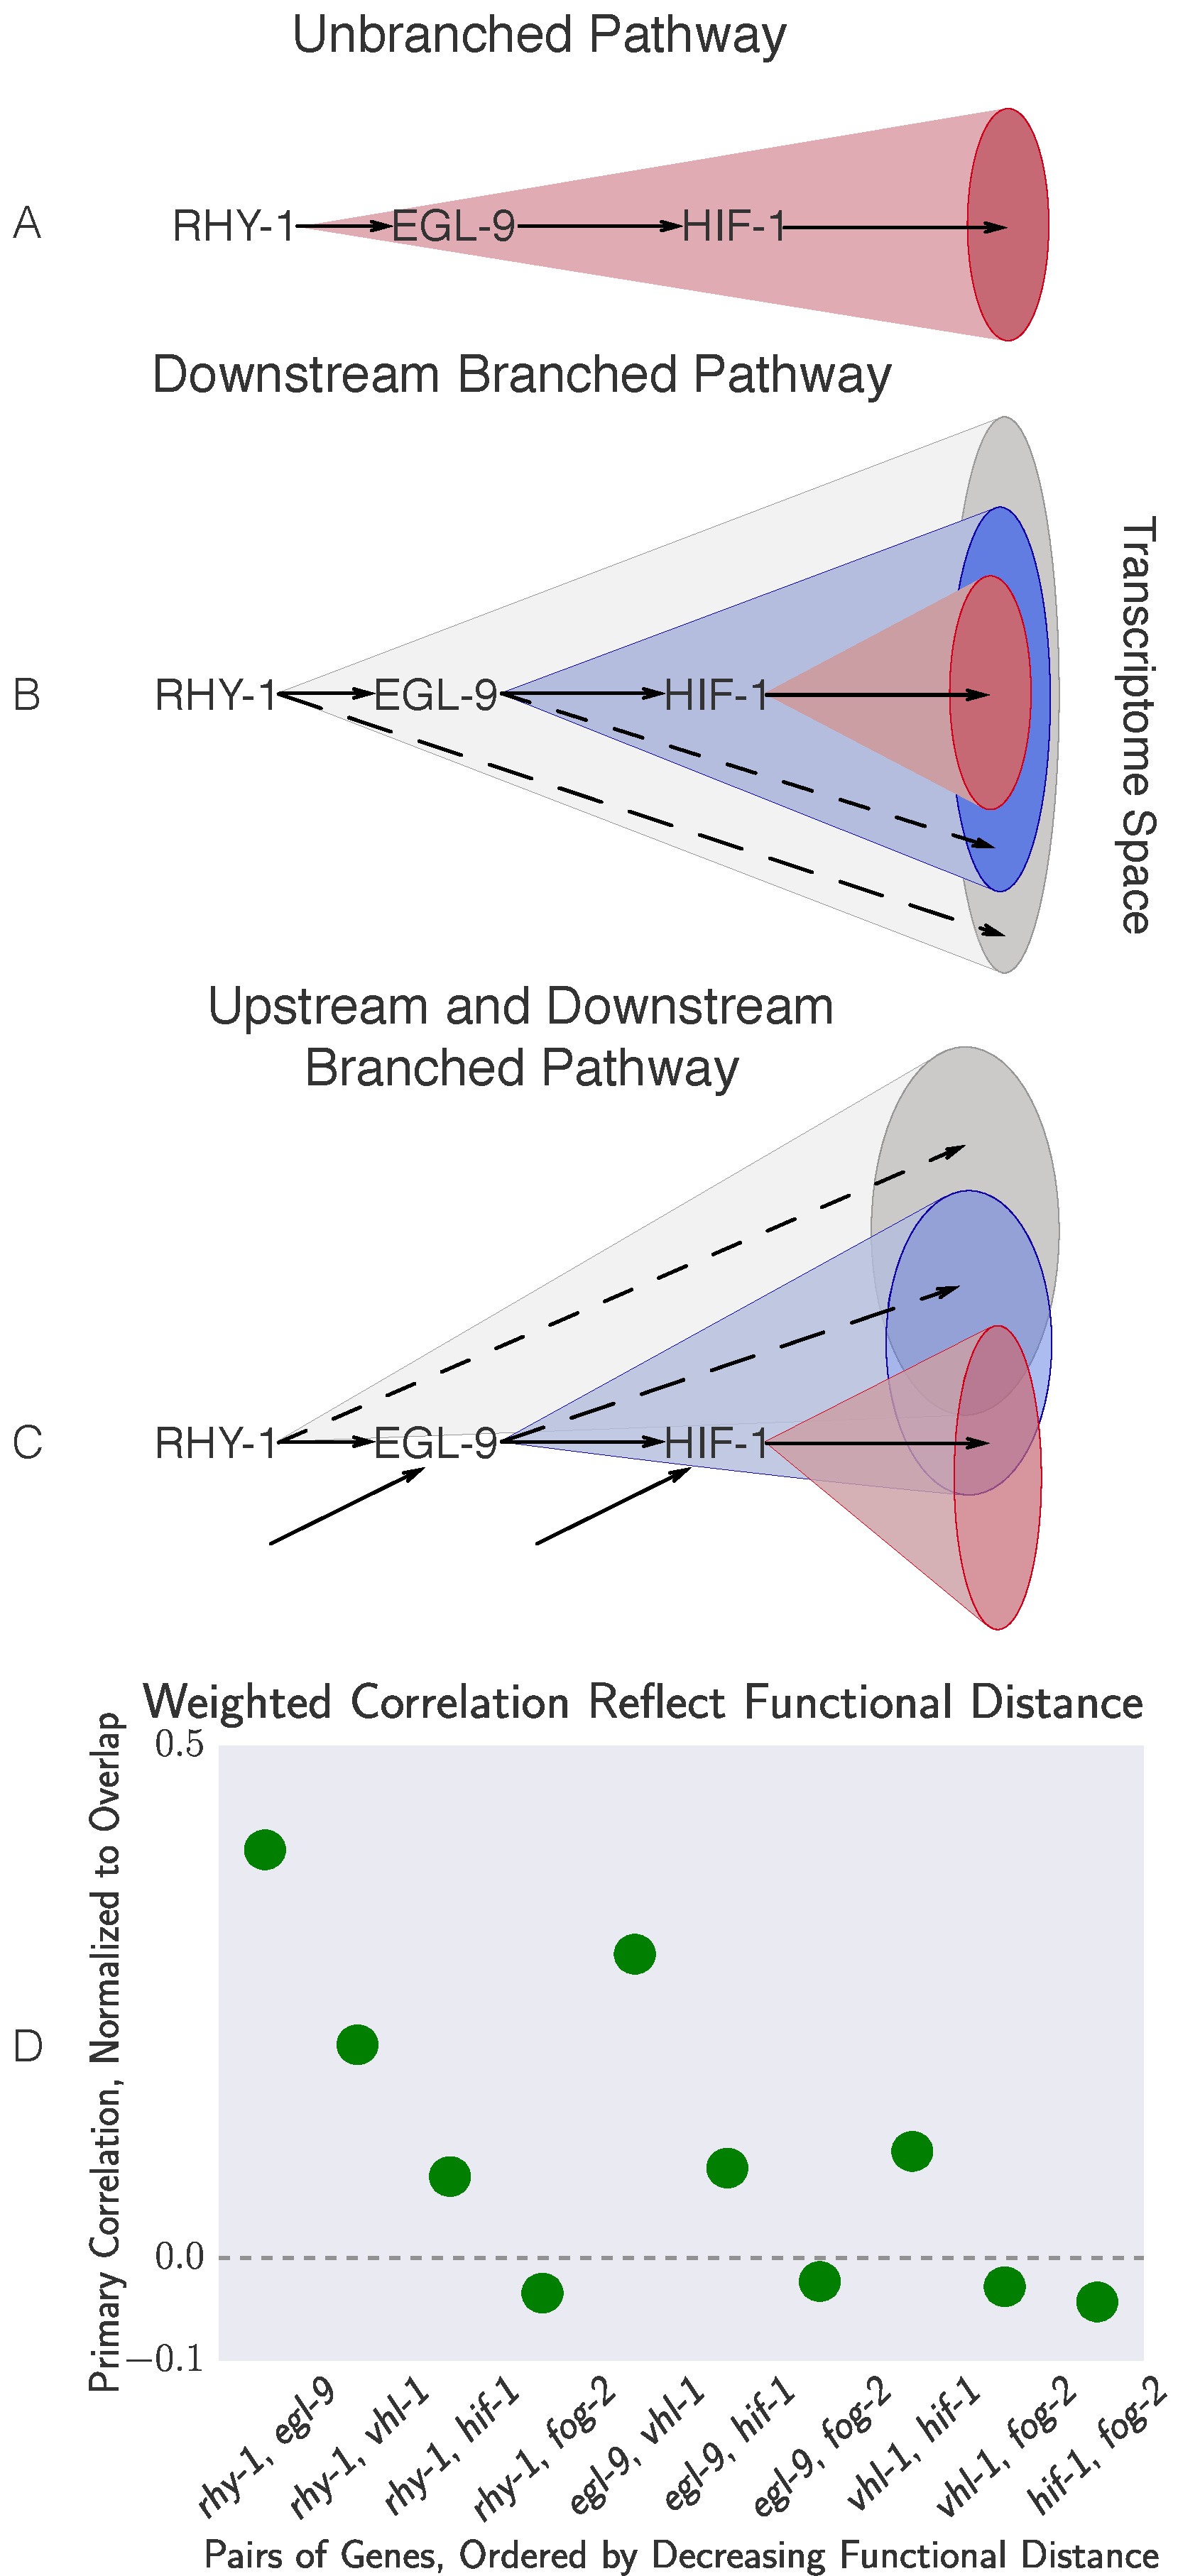
\includegraphics[width=\linewidth]{figs/decorrelation.pdf}
\caption{
Theoretically, transcriptomes can be used to order genes in a pathway under
certain assumptions. Arrows in the diagrams above are intended to show the
direction of flow, and do not indicate valence.
\textbf{A} A linear pathway in which \gene{rhy-1} is the only gene controlling
\gene{egl-9},
which in turn controls \gene{hif-1} does not contain transcriptomes with enough
information to infer the order between genes.
\textbf{B} On the other hand, if \gene{rhy-1} and \gene{egl-9} have transcriptomic
effects that are separable from \gene{hif-1}, then the \gene{rhy-1} transcriptome
should contain contributions from \gene{egl-9}, \gene{hif-1} and \gene{egl-9}- and
\gene{hif-1}-independent pathways. This pathway contains enough information to
infer order.
\textbf{C} If a pathway is branched in both upstream and downstream directions,
observed transcriptomes will show even faster decorrelation. Nodes that are
separated by many edges may begin to behave almost independently of each other
with marginal transcriptomic overlap or correlation, reflecting the weak control
distant nodes exert on each other.
\textbf{D} The hypoxia pathway can be ordered according to functional distance.
We hypothesize the rapid decay in correlation is probably due to a mixture of
upstream and downstream branching that happens along this pathway.
% At this time, we are unable
% to demonstrate branching in this pathway.
}
\label{fig:decorrelation}
\end{figure}

We investigated the possibility that transcriptomic signals do in fact contain
relevant information about the degrees of separation by weighting the robust
bayesian regression between each pair of genotypes by
$N_\mathrm{Intersection}/N_{\mathrm{Union}}$. We plotted the weighted
correlation of each gene pair, ordered by increasing functional distance
(see Fig.~\ref{fig:decorrelation}). In every case, we see that the weighted
correlation decreases monotonically due mainly, but not exclusively, to
decreasing $N_\mathrm{Overlap}$.
We believe that this result is not due to random noise or insufficiently deep
sequencing. Instead, we propose a framework in which every gene is regulated
by multiple different molecular species, which induces progressive decorrelation.
This decorrelation in turn has two consequences. First, decorrelation within a
pathway implies that two nodes may be almost independent of each other if the
functional distance between them is large. Second, it may be possible to use
decorrelation dynamics to infer gene order in a pathway, as we have done with
the hypoxia
pathway\footnote{
An important question is whether a looped circuit
like the hypoxia pathway can be ordered in the way we have ordered it in
Fig.~\ref{fig:decorrelation} since a loop does not technically have a beginning.
One explanation is that we studied the hypoxia pathway under normoxic conditions,
and therefore the control of \gene{hif-1} over \gene{rhy-1} and \gene{egl-9} is
weak, effectively turning the looped pathway into a linear one. Probably, under
hypoxic conditions the pathway would effectively be reversed.
}.

\subsection*{The circuit topology of the hypoxia pathway explains patterns in
            the data}
\label{sub:topology}
We noticed that while some of the rank-plots contained a clear positive correlation
(see Fig.~\ref{fig:genetic_interactions}), some of the other rank-plots showed
a discernible cross-pattern (see Fig.~\ref{fig:xpattern}). In particular, this
cross-pattern emerged between \vhl{} and \rhy{} or between \vhl{} and \egl{},
even though genetically \gene{vhl-1}, \gene{rhy-1} and \gene{egl-9} are all
inhibitors of \hif{}. We reasoned that it could be possible that these
cross-patterns reflected multiple interaction modes between genes
% : while \vhl{}, \rhy{} and \egl{} are all inhibitors
% of \hif{}, \rhy{} and \egl{} are also genetically activated by \hif{}. Turning
% on the hypoxia response by mutating \vhl{} should increase expression of \rhy{}
% and therefore augment its transcriptional effects; however, turning the hypoxia
% pathway on by mutating \rhy{} would also perturb the transcriptional effects specific
% to \rhy{}.
Therefore, we hypothesized that patterns in the rank-plots contained
valuable information for decoding more interactions in our circuit.

% correlative genetics again
\begin{figure}[tbhp]
\centering
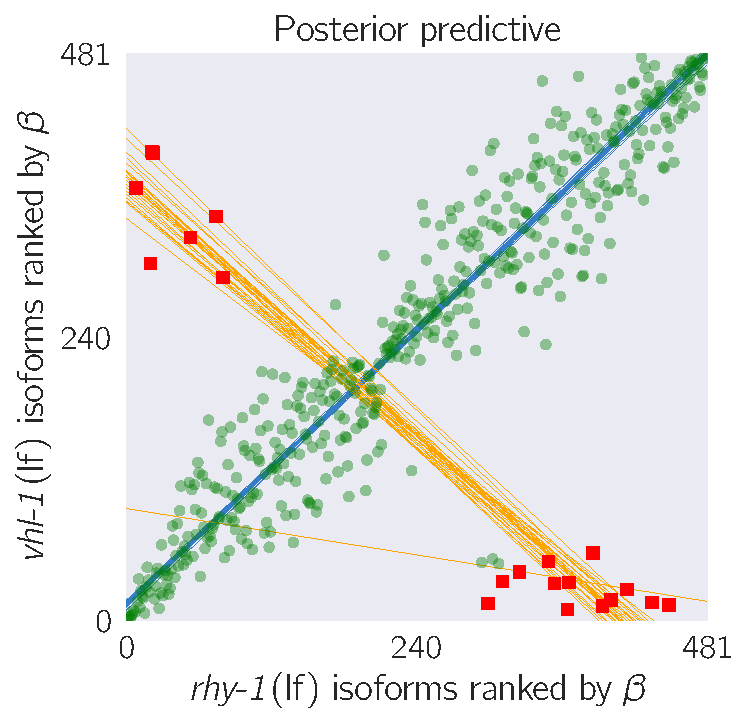
\includegraphics[width=\linewidth]{figs/multiplemodes-ed.pdf}
\caption{
\textbf{Top}: A feedback loop can generate transcriptomes that are both
correlated and anti-correlated. \textbf{Bottom}: \hif{} transcriptome correlated
to the \rhy{} transcriptome. Green large points are inliers to the first
regression. Red squares are outliers to the first regression. Only the red
small points were used for the secondary regression. Blue lines are representative
samples of the primary bootstrapped regression lines. Orange lines are
representative samples of the secondary bootstrapped regression lines.
}
\label{fig:xpattern}
\end{figure}

If the logic above is correct, then it should be possible to decouple
transcriptomes in a logically consistent way. Currently, transcriptomes are
decoupled via subtractive logic. In other words, to identify the
\gene{rhy-1}-specific
transcriptome (the effects of \gene{rhy-1} not dependent on \gene{}egl-9),
subtractive logic
might suggest to find the overlap between the two transcriptomes. The genes that
are differentially expressed but are not in the overlap would then be considered
\gene{rhy-1}-specific transcriptomes. Such a gene set would consider of almost
700 genes. However, this approach suffers from a number of
drawbacks, principally that it does not take into account the relationship
between the two genes in question. Moreover, these genes have no testable properties:
i.e., a gene might not be in the overlap because it was not identified due to
chance in one of the two transcriptomes. In aggreggate, there is no pattern that
is present in these genes that can be used to identify them beyond overlapping
the two transcriptomes.

\gene{rhy-1} and \gene{egl-9} share a well-defined relationship. \rhyp{}
inhibits \cyslp{},
which in turn inhibits \eglp{}~\cite{Ma2012}. Therefore, loss of \rhyp{} leads
to inactivation of \eglp{}, which leads to increase in the cellular levels of
\hifp{}. \hifp{} in turn causes the mRNA levels of \gene{rhy-1} and \gene{egl-9}
to increase,
as they are involved in the \gene{hif-1}-dependent hypoxia response. However, since
\gene{rhy-1} has been mutated, the observed transcriptome is
\rhyp{} `null'; \eglp{} `null'; \hifp{} `on'. The situation is similar for
\egl{}, except that \rhyp{}
is not inactive, and therefore the observed transcriptome is the result of
\rhyp{} `up'; \eglp{} `null'; and \hifp{} `on'. From this pattern, we conclude that
the \egl{} and \rhy{} transcriptomes should exhibit a cross-pattern when plotted
against each other: The positive
arm of the cross is the result of the \eglp{} `null'; \hifp{} `on' dynamics; and the
negative arm reflects the different direction of \rhyp{} activity between
transcriptomes. However, no negative arm is visible (with the exception of two
outliers, which are annotated as pseudogenes in WormBase). Therefore, it is likely
that a large portion or possibly all the transcriptomic effects of \rhyp{} in
this dataset are downstream of \egl{}.

Next, we wanted to know whether our dataset was able to capture
\gene{hif-1}-independent transcriptomic effects of  \gene{egl-9}. We have observed
that \hif{} leads to a modest increase in the transcription of \gene{rhy-1},
from which we concluded that \eglp{} would be more active in the \hif{} mutant
than in the wild-type. Therefore, we searched for genes that were regulated in
opposite manner between \hif{} and \eglhif{}, and that were regulated
in the same direction between the \eglhif{} and \egl{} (or \rhy{}) mutants.
We were only able to find a single gene, \emph{clec-88}, which was down-regulated
in \hif{}, but upregulated in every other mutant we studied. Although
it may be the case that \gene{egl-9} does not have a \gene{hif-1}-independent transcriptomic
phenotype, it is also possible that the change in \hifp{} dosage between a
wild-type normoxic animal and a \hif{} animal is not sufficient to alter the
activity of \eglp{} to a consistently detectable level given our read-depth.
% Due
% to the privileged role of \eglp{} in controlling this circuit, the comparison
% between \hif{} and \egl{};\hif{} animals is the most important comparison for
% identifying an \egl{}-specific transcriptome.

We leveraged this genetic logic to identify a main hypoxia
response induced by removing inhibition on \gene{hif-1} (260 genes). Although the
hypoxic response is likely to involve between five and ten times more genes,
this is a conservative estimate that minimizes false negative results, since
these changes were identified in four independent genotypes with three replicates
each. We also identified a \gene{vhl-1}-specific response, resulting in \vhltargets{}
genes. We searched for candidates directly regulated by \gene{hif-1}.
Initially, we generated this list using the most stringent pattern
matching, but this revealed only 2 genes (\emph{R08E5.3} and
\emph{nit-1}). A relaxed set of conditions (target genes should go up in all
mutants that induce \hifp{}, and should not be up in \hif{}) identified
\hiftargets{} candidate genes.

\subsubsection*{Enrichment analysis of the hypoxia response}
\label{sub:ea_hypoxia}
In order to validate that our transcriptomes were correct, and to understand how
functionalities may vary between them, we subjected each decoupled response to
enrichment analysis using the WormBase Enrichment
Suite~\cite{Angeles-Albores2016}.

\begin{figure}[tbhp]
\centering
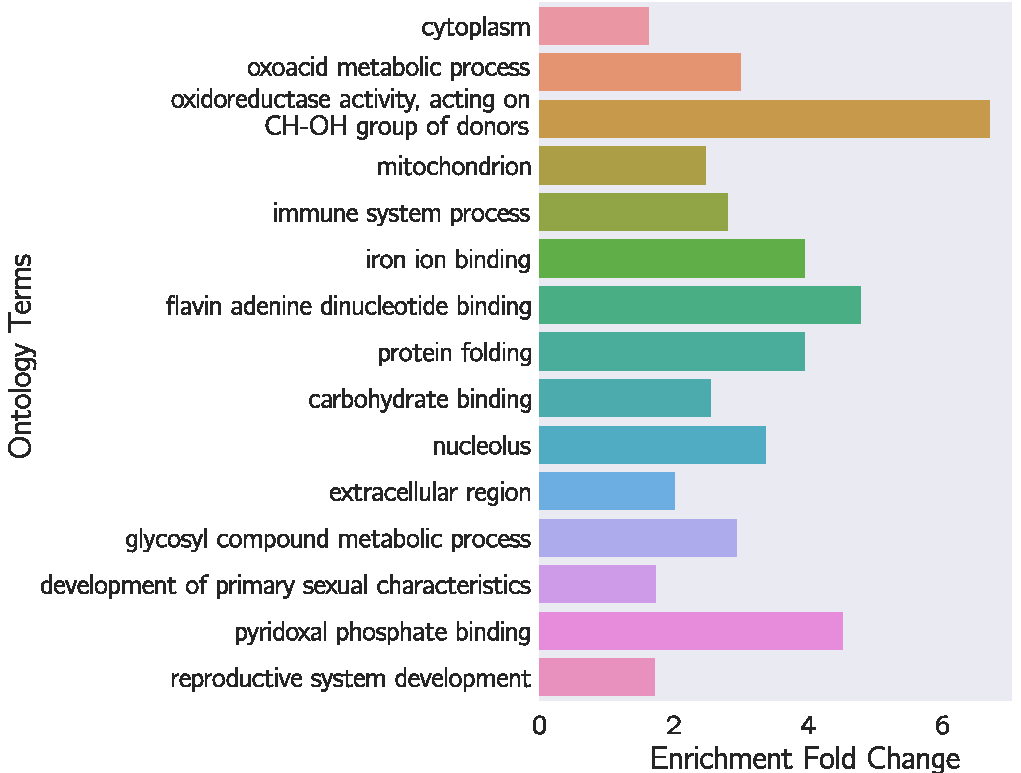
\includegraphics[width=\linewidth]{figs/hypoxia_response_gea.pdf}
\caption{
Gene ontology enrichment analysis of genes associated with the main hypoxia response.
A number of terms reflecting catabolism and bioenergetics are enriched.
}
\label{fig:hyp_gea}
\end{figure}

Gene ontology enrichment analysis (GEA) showed that the terms `oxoacid metabolic process'
(\qval{3}, 3.4 fold-change, 19 genes),
`iron ion binding' (\qval{3}, 5.5 fold-change, 10 genes),
and `immune system process' (\qval{3}, 3.4 fold-change, 17 genes) were enriched
with the lowest q-values. GEA also showed enrichment of terms including
`electron carrier activity' (\qval{1}, 4.8 fold-change, 5 genes),
`mitochondrion' (\qval{2}, 2.5 fold-change, 20 genes)
and `respiratory chain' (\qval{1}, 4.6 fold-change, 4 genes) (see
Fig.~\ref{fig:hyp_gea}). Indeed, \hif{} has been implicated in
all of these biological and molecular functions~\cite{Luhachack2012,Ackerman2012,
Romney2011,Semenza2011}. Phenotype Enrichment Analysis (PEA) revealed that this
gene list was enriched in two phenotypes: `oxygen response variant' (\qval{2},
5.8 fold-change, 7 genes) and `pleiotropic defects severe early embryo' (\qval{2},
4.4 fold-change, 9 genes). The overrepresented terms from PEA and GEA are biologically
directly connected to the process we are studying, which suggests that we have
correctly identified the main hypoxic response. As a final test to guarantee the
quality of our data, we selected a set of 21 known reporters from the literature
and asked whether these reporters were present in our list. We found $5/21$ known
reporters, which constitutes a statistically significant result ($p<10^{5}$).
The small number of reporters found in this list probably reflects the conservative
nature of our estimates. We also analyzed the list of predicted \hifp{} direct targets.
Phenotype Enrichment Analysis revealed that this list was significantly enriched in
`oxygen response variant' (\qval{2}, 12.3 fold-change, 4 genes) and Tissue Enrichment
Analysis (TEA) showed enrichment of the `coelomic system' (\qval{1}, 2.7 fold-change,
16 genes). The \gene{vhl-1}, \gene{hif-1}-independent specific transcriptome was also submitted
for enrichment analysis but no terms were significantly enriched.\todo{closer is missing.}

\subsection{Identification of non-classical epistatic interactions}
\label{sub:hifoh}
\hif{} has traditionally been viewed as existing in a genetic OFF state under
normoxic conditions. However, our dataset indicates that \hifn{} genes show
altered expression when it is removed in normoxic conditions. Moreover, we
observed positive genome-wide expression correlations between \hif{} expression
levels and \egl{}, \vhl{} and \rhy{} expression levels in spite of the negative
regulatory relationships between these genes and \gene{hif-1}. Such positive
relationships could indicate a different relationship between these genes
than has previously been reported. We wanted to explore whether these genome-wide
positive correlations were substantiated by epistasis analyses.

To perform epistasis analyses, we first identified genes that exhibited violations
of the canonical genetic model of the hypoxia pathway. To this end, we searched for
genes that exhibited different behaviors between \egl{} and \vhl{}, or
between \rhy{} and \vhl{} (we assume that all results from the
\rhy{} transcriptome reflect a complete loss of \gene{egl-9} activity). We found
\hifohtargets{} that satisfied this condition (see Fig.~\ref{fig:hif1oh}).
Additionally, many of these genes exhibited new kinds of epistasis. Namely,
\gene{egl-9} was epistatic over \gene{vhl-1}. Identification of a set of genes
that have a consistent set of relationships with between themselves suggests that
we have identified a new aspect of the hypoxia pathway.

\begin{figure}[tbhp]
\centering
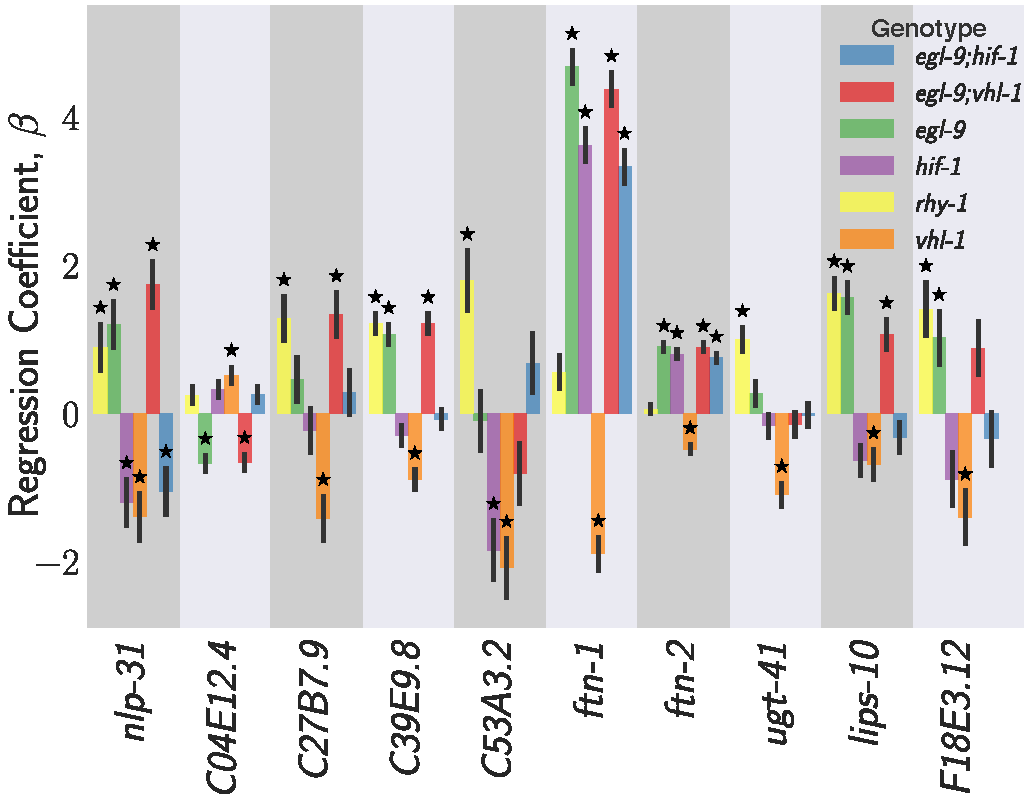
\includegraphics[width=\linewidth]{figs/hif1oh_epistasis.pdf}
\caption{
(\textbf{A}) 27 genes in \cel{} exhibit non-classical epistasis in the hypoxia
pathway, characterized by an opposite phenotypes of the \vhl{} and \egl{} (or
\rhy{}) mutants. Shown are a random selection of the 27 genes for illustrative
purposes.
(\textbf{B}) Representative genes showing that non-canonical epistasis shows a
consistent pattern. \vhl{} mutants have an opposite effect to \egl{}, but
\gene{egl-9} remains epistatic to \gene{vhl-1} and loss of function mutations in
\gene{hif-1} suppress the \egl{} phenotype.
}
\label{fig:hif1oh}
\end{figure}

In particular, we focused on three genes, \nlp{}, \ftna{} and \ftnb{}, which
epistasis patterns that we felt reflected the population well. \ftna{} and \ftnb{}
are both described in the literature as genes that are responsive to mutations in
the hypoxia pathway. Moreover, these genes have been previously described to have
aberrant behaviors~\cite{Ackerman2012,Romney2011}, specifically the
opposite effects of \egl{} and \vhl{}. These studies showed that loss of \vhl{}
suppresses \ftna{} and \ftnb{} using both RNAi and alleles, which allays concerns
of strain-specific interference. Moreover, Ackerman and Gems (2012) showed that
\gene{vhl-1} is epistatic to \gene{hif-1}, and that loss of
\hifp{} is associated with increased expression of \ftna{} and \ftnb{}. We observe
that \gene{hif-1} is epistatic to \gene{egl-9}, and that \gene{egl-9} and
\gene{hif-1} both promote \ftna{} and \ftnb{} expression.
\todo[inline]{see Romney2011 figure 2b; Ackerman2012 Fig. 3; Fig.6}
This further validates the quality of our RNA-seq data and the analysis, and
highlights the power of RNA-seq to identify novel interactions.

Epistasis analysis of \ftna{} and \ftnb{} reveals that \gene{egl-9} is
epistatic to \gene{hif-1}; that \gene{vhl-1} has opposite effects to \gene{egl-9};
and \gene{vhl-1} is epistatic to \gene{egl-9}. Analysis of \nlp{}
reveals similar relationships. \nlp{} expression is decreased in \hif{},
and increased in \egl{}. However, \gene{egl-9} is epistatic to \gene{hif-1}.
Like \ftna{} and \ftnb{},  \gene{vhl-1} has the opposite effect to \gene{egl-9},
yet is epistatic to \gene{egl-9}.

\subsection{Genome-wide effects of \hifp{}}
\label{sub:metabolism}

We identified the transcriptional changes
associated with bioenergetic pathways in \cel{} by extracting from
WormBase all genes associated with the tricarboxylic acid (TCA) cycle, the
electron transport chain (ETC) and with the \cel{} energy reserve (glycogen
metabolism, fatty acid metabolism, etc\ldots). Previous research has described
the effects of mitochondrial dysfunction in eliciting the hypoxia
response~\cite{Lee2010}, but transcriptional feedback from \hifp{} into
bioenergetic pathways has not been as well described in \cel{}, although it has
been extensively described in vertebrates (see, for example~\cite{Semenza1994,
Semenza2012}).
\todo[inline]{I have searched the literature fairly thoroughly, and haven't
seen a complete transcriptional description of hif-1 induced changes in the TCA,
ETC.\@ Can anyone let me know if I missed something?}
We also searched for the changes in ribosomal components and the proteasome, as
well as for terms relating to immune response (see Fig~\ref{fig:genomewide}).

\begin{figure}[tbhp]
\centering
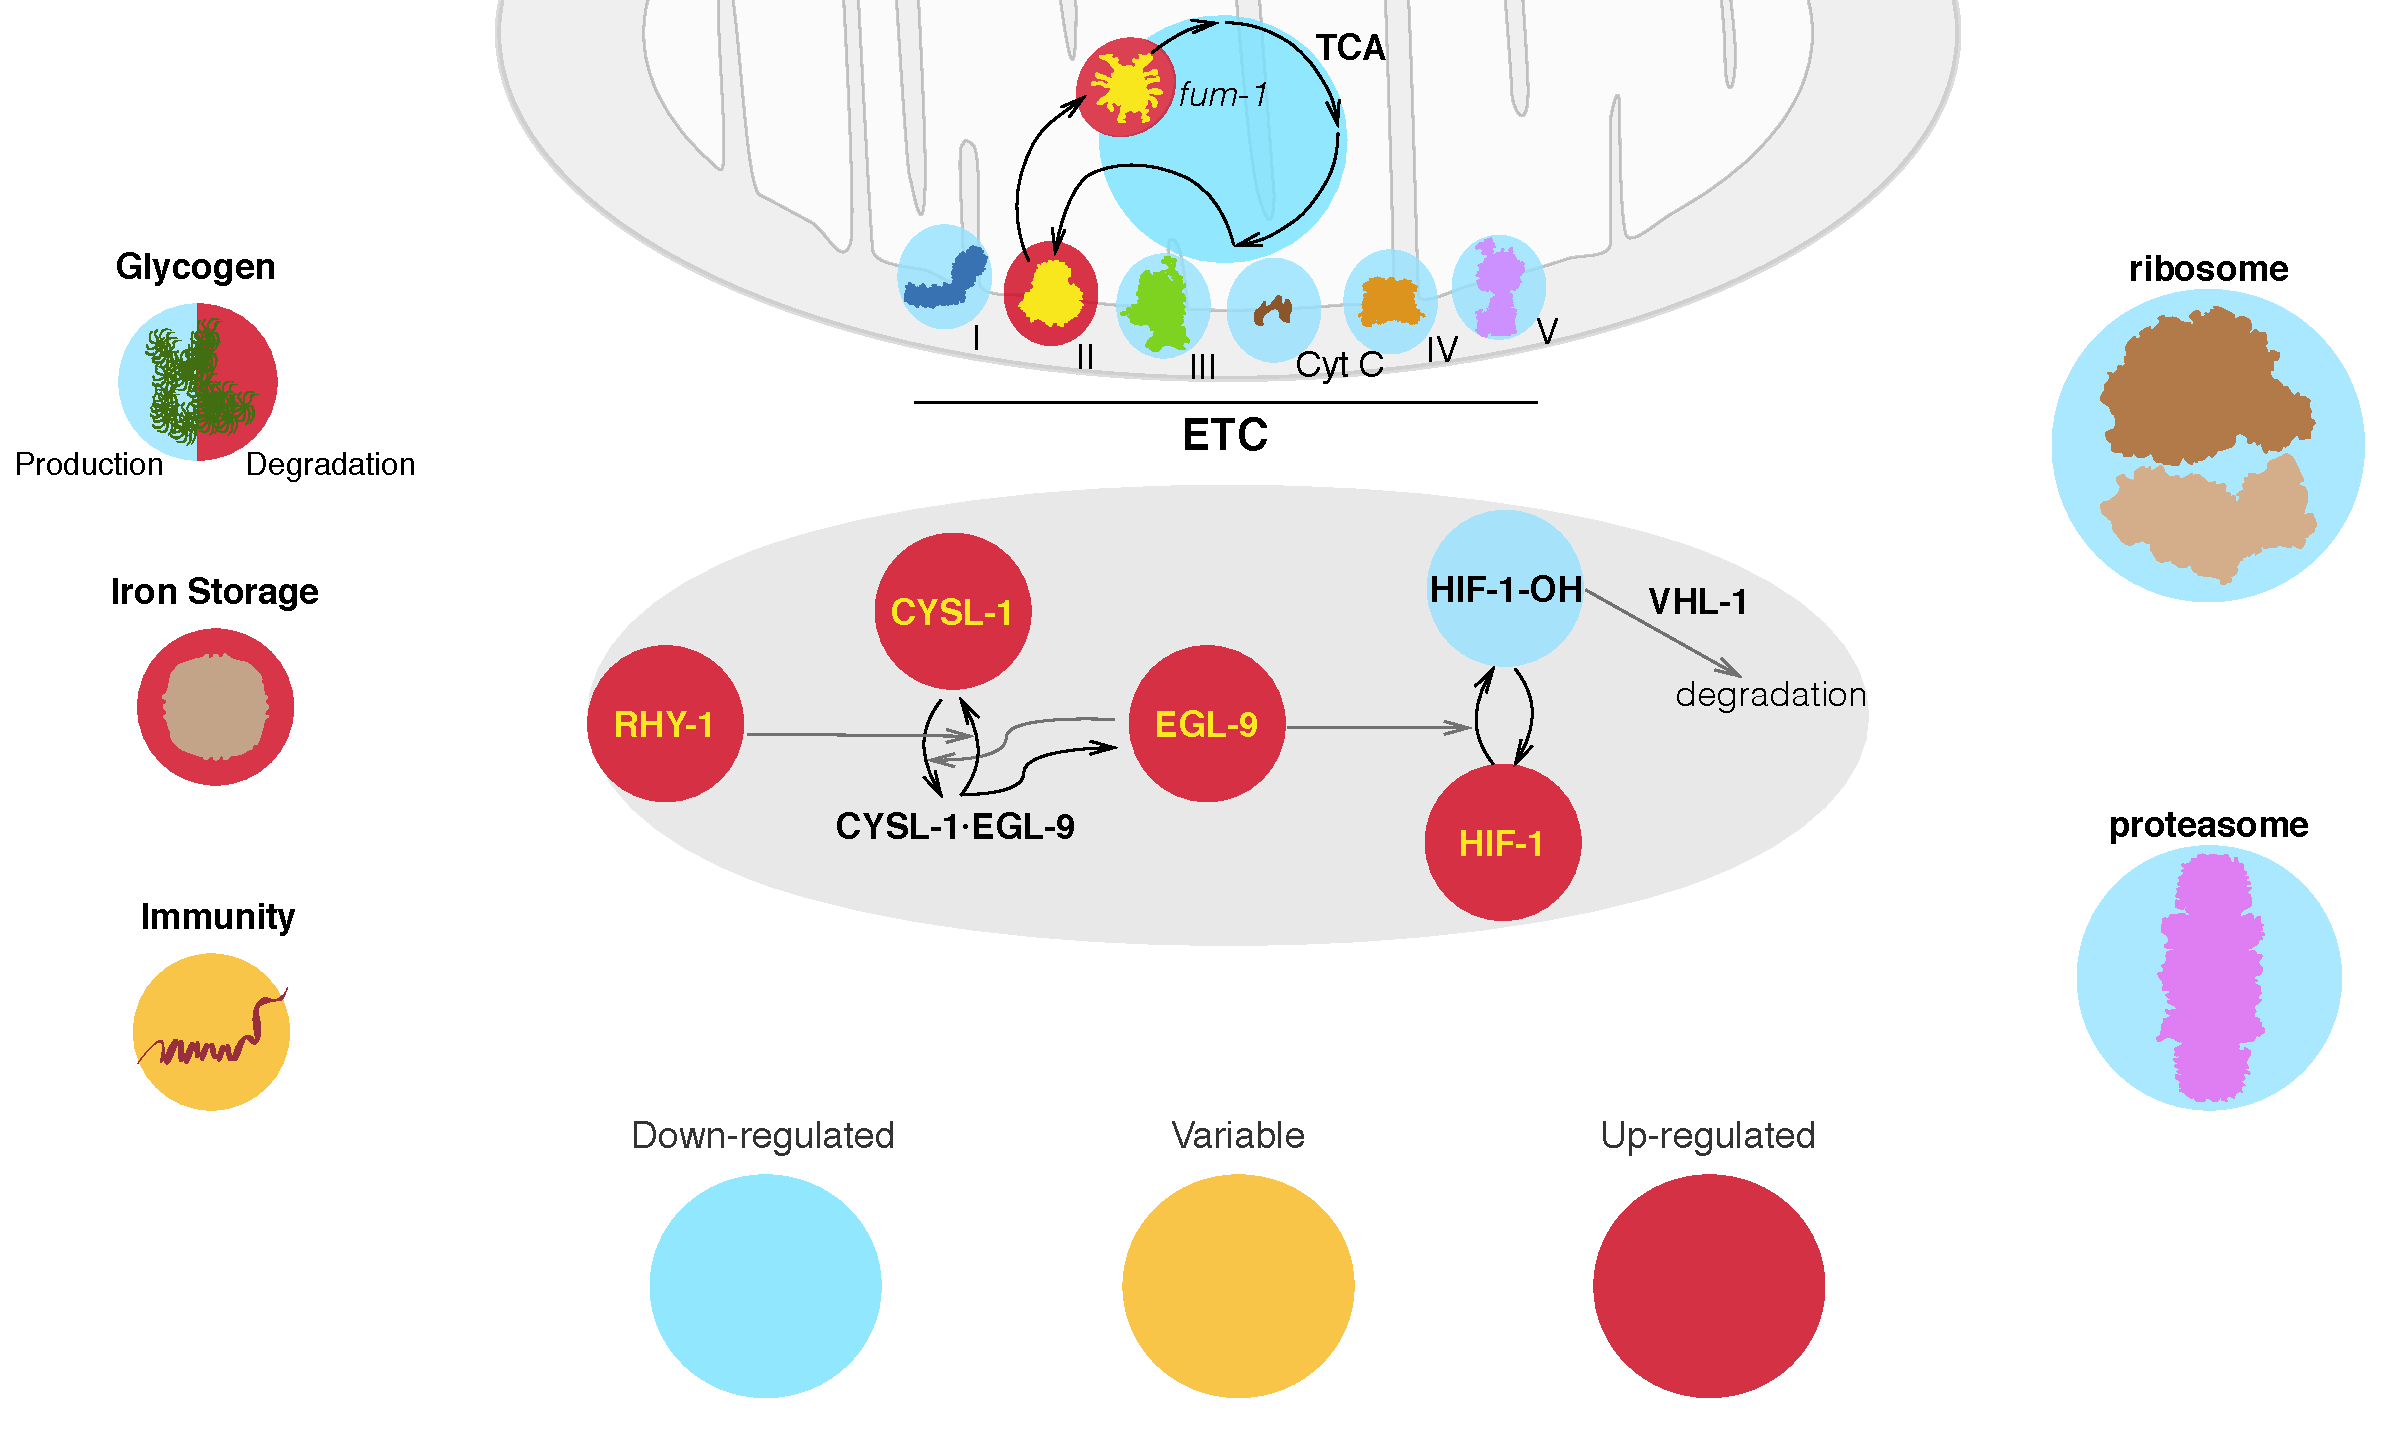
\includegraphics[width=\linewidth]{figs/hif1genomewide.pdf}
\caption{
A graphic summary of the genome-wide effects of \hifp{} from our RNA-seq data.
}
\label{fig:genomewide}
\end{figure}


\subsubsection{Bio-energetic pathways}

\todo[inline]{Bio-energetic or bioenergetic?}
Our data shows that most of the enzymes involved in the TCA cycle and in the ETC
are down-regulated when \hifp{} is induced in agreement with the previous
literature~\cite{Semenza2012}.
\todo[inline]{Missing ETC citation}
However,
\gene{fum-1} and the mitochondrial complex II stood out as notable exceptions to
the trend, as they were up-regulated in every single genotype that causes
deployment of the hypoxia response. \gene{fum-1} catalyses the reaction of
fumarate into malate, and complex II catalyses the reaction of succinate into
fumarate. Complex II has been identified as a source of reserve respiratory capacity
in neonatal rat cardiomyocytes previously~\cite{Pfleger2015}.
\todo[inline]{Missing
discussion of why this is biologically relevant. Fumarate is a poison for egl-9.}
We found two energy reserve genes that were down-regulated by \hifp{}. \gene{aagr-1}
and \gene{aagr-2}, which are predicted to function in glycogen
catabolism~\cite{Sikora2010} were both down-regulated in all the relevant mutants.
Three distinct genes involved in energy reserve were up-regulated. These genes were
\gene{ogt-1}, an O-linled GlcNac Transferase; \gene{T04A8.7}, an ortholog of human
glucosidase acid beta (GBA); and \gene{T22F3.3}, an ortholog of human glycogen
phosphorylase isozymes.

\subsubsection{Protein synthesis and degradation}

\hif{} is also known to inhibit protein synthesis and translation in varied ways.
\hifp{} is known to control the translational machinery indirectly
via inhibition of mTOR~\cite{Brugarolas2004}. However, most reported effects of
\hifp{} on the translation machinery are posttranslational, and no reports to date
show decreases in transcription of the ribosomal machinery in \cel{}. We used
the WormBase Enrichment Suite Gene Ontology dictionary~\cite{} to extract 143 genes
annotated as `structural constituents of the ribosome' and we queried whether they
were differentially expressed in our mutants. \egl{}, \vhl{}, \rhy{} and
\egl{};\vhl{} showed differential expression of 91 distinct ribosomal
constituents (not all constituents were detected in all genotypes). For every one
of these genotypes, these genes were always down-regulated. In contrast,
\hif{} showed up-regulation of a single ribosomal constituent.

Next, we asked whether \hifp{} has any transcriptional effects on the
proteasomal constituents, because no such effects of \hifp{} on the proteasome
have been reported in \cel{}. Out of 40 WormBase annotated proteasomal constituents,
we found 31 constituents that were differentially expressed in at least one of the
four genotypes that induce a hypoxic response. Every gene we found was down-regulated
in at least two out of the four genotypes we studied, although in each case the
down-regulation was minor.
% It is impossible to distinguish whether these animals
% exhibit a decrease in proteasome expression is due to a lower requirement for
% degradation in these animals due to constitutively depressed translation rates or
% whether the decrease in expression is a direct result of \hifp{} stabilization.

\section*{Discussion}
\subsection*{The \cel{} hypoxia pathway can be reconstructed entirely from
             RNA-seq data}
In this paper, we have shown that transcriptomic phenotypes using whole-organism
RNA-seq can be used to reconstruct genetic pathways. We reconstructed the
pathway to first- and second- order interaction between genes in the pathway.
We inferred order of action (\gene{rhy-1} activates \gene{egl-9}, \gene{egl-9} and
\gene{vhl-1} inhibit \gene{hif-1}), and we were able to infer from genome-wide
epistasis measurements that \gene{egl-9} exerts \gene{vhl-1}-dependent and
independent inhibition on \gene{hif-1}.

\subsection*{\hifp{} and the cellular environment}

In addition to reconstructing the pathway, our dataset allowed us
to observe a wide variety of physiologic changes that occur as a result of the
\hifp{}-dependent hypoxia response. In particular, we observed down-regulation of most
components of the TCA cycle and the mitochondrial electron transport chain with
the exceptions of \gene{fum-1} and the mitochondrial complex II.\@ The mitochondrial
complex II catalyses the reaction of succinate into fumarate. Complex II is known
to be important for hypoxic survival in rat cardiomyocyte cells~\cite{Pfleger2015}.
Complex II may play a similar role in \cel{}. However, the product of complex II
activity is fumarate. In mouse embryonic fibroblasts, fumarate has been
shown to antagonize \hifp{} prolyl hydroxylase domain (PHD) enzymes, which are
orthologs of \eglp{}~\cite{Sudarshan2009}. Upregulation of complex II by \hifp{}
during hypoxia may therefore result in increased intracellular levels of fumarate,
which in turn could lead to artificially high levels of \hifp{} (if the inhibitory
role of fumarate is conserved in \cel{}) even after normoxia resumes. The increase
in fumarate produced by the complex could be compensated by increasing expression of
\gene{fum-1}. Increased fumarate degradation allows \cel{} to maintain plasticity
in the hypoxia pathway, keeping the pathway sensitive to oxygen levels.

\subsection*{Non-classical epistasis in the hypoxia pathway}
The observation of almost 30 genes that exhibit a specific pattern of non-classical
epistasis suggests new aspects of the hypoxia pathway. Some of these non-classical
epistases had been observed previously, but no satisfactory mechanism has been
proposed to explain this biology. \citep{Romney2011} and \citep{Ackerman2012}
suggest that \hifp{} integrates information on iron concentration in the
cell to bind to the \ftna{} promoter, but could not definitively establish
a mechanism.
It is unclear why deletion of \gene{hif-1} induces \ftna{}
expression, deletion of \gene{egl-9} also causes induction of \ftna{} expression,
but deletion of \gene{vhl-1} removes this inhibition. Moreover, \citep{Luhachack2012}
have previously reported that certain genes important for the \cel{} immune response
against pathogens reflect similar expression patterns. Their interpretation
was that \gene{swan-1}, a binding partner to \eglp{}~\cite{Shao2010}, is important
for modulating \hifp{} activity in some manner. The lack of a conclusive double
mutant analysis in this work means the role of SWAN-1 in modulation of
\hifp{} activity remains to be demonstrated.
At any rate, mechanisms that call for additional
transcriptional modulators become more unlikely given our data the large number of
genes with different biological functions that exhibit the same pattern.

\begin{figure}[tbhp]
\centering
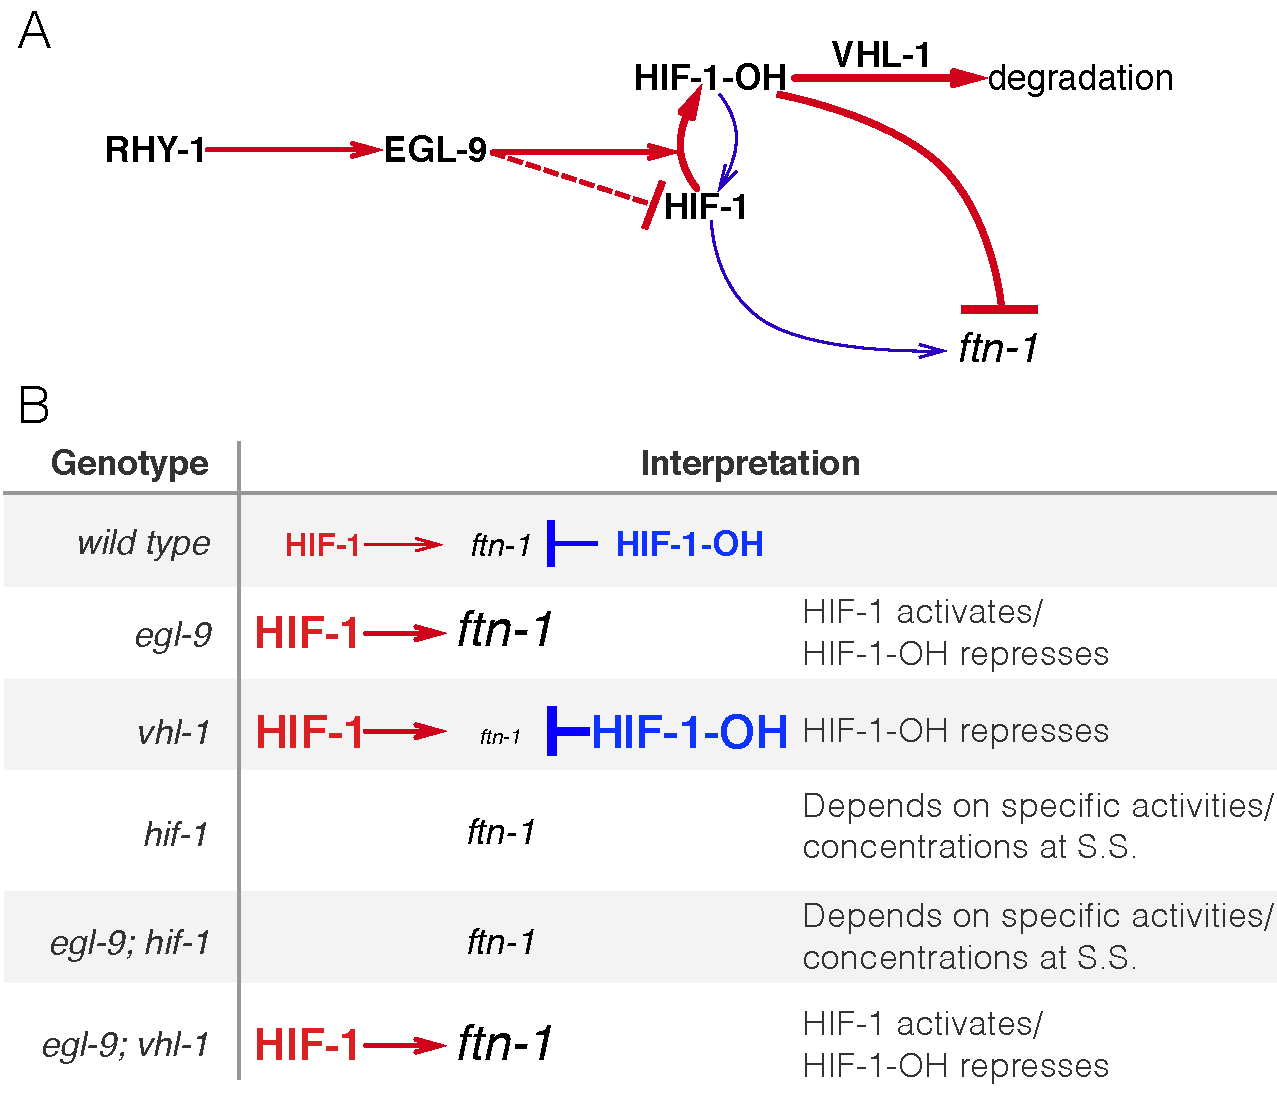
\includegraphics[width=\linewidth]{figs/hif1oh_model.pdf}
\caption{
A hypothetical model showing a mechanism where \hifp{}-hydroxyl antagonises
\hifp{}. Such a mechanism can potentially explain how genes that exhibit
non-canonical epistasis are regulated.
}
\label{fig:hif1oh_table}
\end{figure}

One way to resolve this problem without invoking additional genes is to
consider \hifp{} as a protein with both activating and inhibiting states. In fact,
\hifp{} already exists in two states in \cel{}: unmodified \hifp{} and
\hifp{}-hydroxyl (\hifp{}-OH). Under this model, \hifp{}-hydroxyl antagonizes
the effects of \hifp{} for certain genes like \ftna{} or \nlp{}. Loss of
\gene{vhl-1} stabilizes \hifp{}-hydroxyl.
A subset of genes that are sensitive to \hifp{}-hydroxyl will be inhibited as a
result of the increase in the amount of this species, in spite of the increased
levels of \hifp{}.
On the other hand, \egl{} selectively removes all \hifp{}-hydroxyl, stimulating
accumulation of \hifp{} and promoting gene activity. Whether deletion of \hif{}
is overall activating or inhibiting will depend on the relative activity of each
protein state under normoxia (see Fig.~\ref{fig:hif1oh_table}).

The possibility that \hifp{}-hydroxyl has a function has not been previously
considered in the existing literature, although experts have wondered about
the possibility that \hifp{}-hydroxyl may have transcriptional effects independent
of \hifp{} (William Kaelin, pers.\ comm.). \todo[inline]{Paul, do we need to ask
W. K. for permission to cite? } Varied lines
of circumstantial evidence that \hifp{} hydroxylation plays a role
in the functionality of the hypoxia pathway. First, \hifp{}-hydroxyl is
challenging to study genetically because no mimetic mutations are available with
which to study the pure hydroxylated \hifp{} species. Second, although mutations in
the Von-Hippel Landau gene stabilize the hydroxyl species, they also increase the
quantity of \hifp{} by mass action. Finally, since \hifp{} is detected low levels
in cells under normoxic conditions~\cite{Wang1993}, total \hifp{} protein
(unmodified \hifp{} plus \hifp{}-hydroxyl) is often tacitly assumed to be
vanishingly rare and therefore biologically inactive.

Our data show hundreds of genes that change expression in response
to loss of \gene{hif-1} under normoxic conditions. This establishes that there is
sufficient total \hifp{} protein to be biologically active.
Our analyses also revealed that \hif{} shares
positive correlations with \egl{}, \rhy{} and \vhl{}, and that each of these genotypes
also shows a secondary negative rank-ordered expression correlation with each other.
These cross-patterns between all loss of function of inhibitors of \hifp{} and
\hif{} can be most easily explained if \hifp{}-hydroxyl is biologically active.

A homeostatic argument can be made in favor of the activity of \hifp{}-hydroxyl.
At any point in time, the cell must measure the levels of
multiple metabolites at once. The \gene{hif-1}-dependent hypoxia
response integrates information from O$_2$, $\alpha$-ketoglutarate
(2-oxoglutarate) and iron concentrations in the cell. One way to
integrate this information is by encoding it only in the effective hydroxylation
rate of \hifp{} by \eglp{}. Then the dynamics in this system will evolve
exclusively as a result of the total amount of \hifp{} in the cell. Such a system
can be sensitive to fluctuations in the absolute concentration of
\hifp{}~\cite{Goentoro2009a}. When the system is in normoxic conditions, when
absolute levels of \hifp{} are low, small fluctuations in copy-number could lead
to partial activation of the hypoxic response due to random change for genes
that are under strong control by \hifp{}. On the other hand, genes that have a low
affinity for \hifp{} will not be affected by these small fluctuations.

For yet other set of genes that must change expression in response to the hypoxia
pathway, it may not make as much sense to integrate metabolite information
exclusively via \eglp{}-dependent hydroxylation of \hifp{}. In particular, genes
that may increase survival in mild hypoxia may benefit from regulatory mechanisms
that are robust to transient changes in protein copy number. Likewise,
genes that are involved in iron or $\alpha$-ketoglutarate metabolism
(such as \ftna{}) may benefit from being able to sense, accurately, small and
consistent deviations from basal concentrations of these metabolites. For these
genes, the information may be better encoded by using \hifp{} and
\hifp{}-hydroxyl as an activator/repressor pair. Such paradoxical circuits are
known to possess distinct advantages for controlling output in a manner that
is robust to transient fluctuations in the levels of their
components~\cite{Hart2012,Hart2013}.

Our RNA-seq data suggests that one of the targets that \hifp{} may target
paradoxically is \rhyp{}. Although \gene{rhy-1} does not exhibit non-classical
epistasis, \hif{} and \eglhif{} both had increased expression levels of \gene{rhy-1}.
We speculate that if \gene{rhy-1} is controlled by both \hifp{} and \hifp{}-hydroxyl,
then this might imply that \hifp{} regulates the expression of its pathway (and
therefore itself) in a manner that is robust to total \hifp{} levels.

% \subsection{Looking forward}
% We have demonstrated the first complete reconstruction of a genetic pathway using
% whole-organism RNA-seq in a complex multicellular organism. Future work must
% rigorously demonstrate that macroscopically derived genetic rules of interaction
% hold genome-wide, and if not, how genetic rules deviate from expectations.


\matmethods{
\label{methods}
\subsection*{Nematode strains and culture}
Strains used were N2 wild-type Bristol, CB5602 \vhl{} (ok161), CB6088
\egl{} (sa307) \hif{} (ia4), CB6116 \egl{} (sa307) \vhl{} (ok161), JT307
\egl{} (sa307), ZG31 \hif{} (ia4), RB1297 \rhy{} (ok1402).
ZG31\hif{} (ia4) is a null mutant of \hif{} which deletes 1231 bp of the second,
third and fourth exons.
JT307 contains the null mutant \egl{} (sa307) which is a  243 bp deletion.
RB1297 contains null mutation \rhy{} (ok1402) with an estimated 700 bp deletion
constructed by the OMRF Knockout Group. CB5602 contains the deletion mutation of
\vhl{} (ok161).
CB6088 contains \egl{} (sa307);\hif{} (ia4). % and was constructed by J.~Hodgkin.
CB6116 contains \egl{} (sa307) \vhl{} (ok161). % and was constructed by J.~Hodgkin.
All strains were provided by the CGC, which is funded by NIH Office of Research
Infrastructure Programs (P40 OD010440).  All lines were grown on standard
nematode growth media (NGM) plates with seeded with OP50 \ecol{} at 20\degree{}C
(Brenner 1974).

\subsection*{RNA Isolation}
Unsynchronized lines were grown on NGM plates at 20C and eggs harvested by
sodium hypochlorite treatment. Eggs were plated on 6 to 9 small 5cm NGM plates
with ample OP50 \ecol{} at a density chosen to avoid starvation and grown at
20\degree{}C.  Worms were staged and harvested based on the time after plating,
vulva morphology and the absence of eggs.  Approximately 30--50 non-gravid young
adults (YA) were picked and placed in 100$\mu$L of TE pH 8.0 at 4\degree{}C in
$0.2$mL PCR tubes.   After settling and a brief spin in microfuge approximately
$80\mu$L of TE was removed from the top of the sample and individual replicates
were snap frozen in liquid N2. These replicate samples were then digested with
Proteinase K for 15min at 60\degree{} in the presence of 1\% SDS and 1.25$\mu$L
RNA Secure (Ambion AM 7005). RNA samples were then taken up in 5 Volumes of
Trizol (Tri Reagent Zymo Research) and processed and treated with DNAase I using
Zymo MicroPrep RNA Kit (Zymo Research Quick-RNA MicroPrep  R1050).
RNA was eluted in dH2O and divided into aliquots and stored at -80\degree{}C.
One aliquot of each replicate was analyzed by both NanoDrop for impurities,
Qubit for concentration and then analyzed on an Agilent 2100 BioAnalyzer.
Replicates were selected that had RNA integrity numbers (RIN) equal or greater
than 9.0 and showed no evidence of bacterial ribosomal bands, except for the
ZG31 mutant where one of three replicates had a RIN of 8.3.

\subsection*{Library Preparation and Sequencing}
10 ngs of quality checked (RIN > 9.0), total RNA from each sample were
reverse-transcribed into cDNA using the Clontech SMARTer Ultra Low Input RNA for
Sequencing v3 kit reagents (catalog \#634848) in the SMARTSeq2 protocol
~\cite{Picelli2014}.  RNA was denatured at 70C for 3 minutes
in the presence of dNTPs, oligo dT primer and spiked-in quantitation standards
(NIST/ERCC from Ambion, catalog \#4456740).  After chilling to 4C, the first
strand reaction was assembled using the LNA TSO primer described in \citep{Picelli2014},
and run at 42C for 90 minutes, followed by denaturation at 70C for 10
minutes.  The entire first strand reaction was then used as template for 13
cycles of PCR using the Clontech v3 kit.  Reactions were cleaned up with 1.8X
volume of Ampure XP SPRI beads (catalog \#A63880) according to the manufacturer’s
protocol.  After quantification using the Qubit High Sensitivity DNA assay, a 3ng
aliquot of the amplified cDNA was run on the Agilent HS DNA chip to confirm the
length distribution of the amplified fragments.  The median value for the
average cDNA lengths from all length distributions was 1076bp.  Tagmentation of
the full length cDNA for sequencing was performed using the Illumina/Nextera DNA
library prep kit (catalog \#FC-121-1030).  Following Qubit quantitation and
Agilent BioAnalyzer profiling, the tagmented libraries were sequenced.
Libraries were sequenced on Illumina HiSeq2500 in single read mode with the read
length of 50 nt to an average depth of 15 million reads per sample following
manufacturer's instructions. Base calls were performed with RTA 1.13.48.0
followed by conversion to FASTQ with bcl2fastq 1.8.4. Spearman correlation of
the transcripts per million (TPM) for each genotype showed that every pairwise
correlation within genotype was $>0.9$.

\subsection*{Read Alignment and Differential Expression Analysis}
We used Kallisto to perform read pseudo-alignment and performed differential
analysis using Sleuth. We fit a generalized linear model for a transcript $t$ in
sample $i$:

\begin{equation}
  y_{t,i} = \beta_{t, 0} + \beta_{t, genotype}\cdot{}X_{t, i} +
  \beta_{t, batch}\cdot{}Y_{t, i} + \epsilon_{t, i}
\end{equation}

where $y_{t, i}$ are the logarithm transformed counts; $\beta_{t, genotype}$ and
$\beta_{t, batch}$ are parameters of the model, and which can be interpreted as
biased estimators of the log-fold change; $X_{t, i}, Y_{t, i}$ are indicator
variables describing the conditions of the sample; and $\epsilon_{t, i}$ is the
noise associated with a particular measurement.

\subsection*{Genetic Analysis, Overview}
Genetic analysis of the processed data was performed in Python 3.5. Our scripts
made extensive use of the Pandas, Matplotlib, Scipy, Seaborn, Sklearn, Networkx,
Bokeh, PyMC3, and TEA libraries~\cite{Team2014,McKinney2011,Oliphant2007,
Pedregosa2012,Salvatier2015,VanDerWalt2011,Hunter2007,Angeles-Albores2016,Waskom}.
Our analysis is available in a Jupyter Notebook~\cite{Perez2007}. All code and
required data (except the raw reads) are available at
\url{https://github.com/WormLabCaltech/mprsq} along with version-control
information. Our Jupyter Notebook and interactive graphs for this project can be
found at \url{https://wormlabcaltech.github.io/mprsq/}. Raw reads were deposited
at XXXXXXXXXXX


\subsection*{Weighted Correlations}
Pairwise correlations between transcriptomes where calculated by first identifying
the set of differentially expressed genes (DEGs) common to both transcriptomes under
analysis. DEGs were then rank-ordered according to their regression coefficient,
$\beta$. Bayesian robust regressions were performed using a Student-T distribution.
Bayesian analysis was performed using the PyMC3 library~\cite{Salvatier2015}
(\texttt{pm.glm.families.StudenT} in Python). If the correlation has an average
value >1, the correlation coefficient was set to 1.

Weights were calculated as the proportion of genes that were $<1.5$ standard deviations
away from the primary regression out of the entire set of shared DEGs for each
transcriptome.

\subsection*{Epistasis Analysis}
For a double mutant $X^-Y^-$, we used the single mutants $X^-$ and $Y^-$ to
find expected value of the coefficient for a double mutant under an additive model
for each isoform $i$.
Specifically,
\begin{equation}
  \beta_{\mathrm{Exp},i} = \beta_{X,i} + \beta_{Y,i}.
\end{equation}

Next, we found the deviation of the double mutant from the additive model ($\delta$)
for each isoform $i$:
\begin{equation}
  \Delta_i = \beta_{XY,i} - \beta_{\mathrm{Exp},i}
  \label{eq:deviation}
\end{equation}

To calculate the genome-wide epistasis coefficient, we plotted
($\beta_{\mathrm{Exp},i}, \Delta_i$) and found the line of best fit using
orthogonal distance regression using the scipy.odr package. We performed a
parametric bootstrap sampling the ordered tuples with replacement using 5,000
iterations to generate a probability distribution of slopes of best fit.

To understand the epistatic relationships completely, we needed to simulate the
possible relationships.
There are as many models as epistatic relationships. The epistatic relationships
are such that:

\begin{equation}
  X^-Y^- = Z,
\end{equation}

where $Z$ is some combination of $X^-$ and $Y^-$. Specifically, $Z$ can take on
the values $X^-$ (X is epistatic to Y); $Y^-$ (Y is epistatic to X);
$X^- + Y^-$ (additive); $k^-, k^-=X^-=Y^-$ (unbranched pathway) and
$X^-, Y^-=WT$ (strong repression, where $Y^-$ is wild-type).

For each case, we modified equation~\ref{eq:deviation}:
\begin{equation}
  \Delta_{Z,i} = \beta_{Z,i} - \beta_{\mathrm{Exp},i}.
\end{equation}

In each case, $\Delta_{Z,i}$ reduces to $-\beta_{X,i}$ or $-\beta_{Y,i}$. For each
model, we performed parametric bootstraps as previously described to generate
probability distributions for each model.

We tested whether a given model could be rejected by identifying the fraction
of the slopes that were equal to a critical value $x$ or more extreme under the model.
Models were rejected if $p<0.05$.


}

\showmatmethods{}% Display the Materials and Methods section

\acknow{
This work was supported by HHMI with whom PWS is an investigator
and by the Millard and Muriel Jacobs Genetics and Genomics Laboratory at
California Institute of Technology.
This article was written with support of the Howard Hughes Medical Institute.
We thank Hillel Schwartz for his help in the fun analysis of ftn-1 epistasis.
We would like to thank Jonathan Liu, Han Wang, and Porfirio Quintero for helpful
discussion.
}

\showacknow{} % Display the acknowledgments section

% \pnasbreak splits and balances the columns before the references.
% If you see unexpected formatting errors, try commenting out this line
% as it can run into problems with floats and footnotes on the final page.
% \pnasbreak{}

% Bibliography
\bibliography{citations}

\end{document}
